\documentclass{article}
\usepackage[utf8]{inputenc}
\usepackage{geometry}
\usepackage{varwidth}
\usepackage{graphicx, subcaption}
\usepackage{amsmath}
\usepackage{enumitem}
\usepackage[toc, page]{appendix}
\usepackage{natbib}
\usepackage{titling}
\usepackage{hyperref}
\usepackage{comment}
\renewcommand\maketitlehooka{\null\mbox{}\vfill}
\renewcommand\maketitlehookd{\vfill\null}

\graphicspath{ {./pictures/} }
\geometry{
a4paper,
total={170mm,237mm},
left=20mm,
top=30mm,
}


\title{Assignment 1 \\ Computing the area of the Mandelbrot set \\ \large Stochastic Simulation \\University of Amsterdam\\
\href{https://github.com/vdesgrange/Stochastic_simulation_project}{https://github.com/vdesgrange/Stochastic\_simulation\_project}}
\author{James Kingsbury (13437542), Viviane Desgrange (13337688) }
\date{17th November 2020}

\begin{document}

    \begin{titlingpage}
        \maketitle
    \end{titlingpage}


    \section*{Abstract}

    The Mandelbrot set is an important topic of study in complex dynamics both for its aesthetic appeal and as an example of a complex structure arising from the application of simple rules. The mathematical properties of the set were formalised in (Doudy, Hubbard and Lavaurs, 1984), building upon work on the parameter space of quadratic polynomials in (Mandelbrot, 1980). The exact area of the set is still an open research question and approaches such as series calculations, area of periodic components and pixel counting have been used in attempts to gain a more accurate estimate. In this report we will explore the properties of the Mandelbrot set, estimate its area with Monte Carlo integration methods, experiment with different sampling methods and explore the use of randomised low-discrepancy sequences.

    \section*{Introduction}

    We will start by studying the theory behind the Mandelbrot set and the implications this theory has for the methodology used to implement an approximation of the area of the set. An adequate review of the set's properties will allow us to properly interpret the results of our experiment and some design choices in our algorithms will depend on domain knowledge relevant to the set. We will also visiualise the set and understand if convergence of points from different regions of the set tend to have different convergence properties (Illustrated in Appendix B).\\
    The second part of the paper will focus on the methodology required to estimate the area of the Mandelbrot set. Therefore, we will study the theory behind Monte-Carlo approach of integration using random numbers, then, we will explain how we use this theoretical method to solve the actual numerical integration problem and investigate the convergence rate of the Monte-Carlo approach for a given number of iterations and samples.\\
    The two final  parts of this paper we will explore variance reduction techniques, allowing us to increase the achievable precision of our area estimates given finite compute power. As the original Monte-Carlo approach considers by default the usage of pure random sampling to estimate integrals, we need to experiment with different sampling methods to understand their influence on on the variance of our estimate. Any output variable of a stochastic simulation (area, in our case) is associated with some variance which limits its precision. To reduce this associated variance, we can apply techniques such as importance sampling, control variets, stratified sampling and quasi-random methods. In this paper we will focus on the latter two techniques. \\
    The algorithms from this assignment are created with help of (Ross, 2013). The algorithms were implemented with the libraries \emph{Numpy} and \emph{SciPy} for fundamental scientific computing methods, as well as \emph{ChaosPy} for uncertainty quantification with Monte-Carlo. Additionally we are using \emph{Matplotlib} library to visualize our results.

    \newpage

    \section{Method}

    \subsection*{Mandelbrot set properties}
    \label{subsection:mandelbrot_theory}
    The Mandelbrot set is the set of complex numbers $c \in \mathbb{C}$ defined by the quadratic recurrence equation:
    \begin{equation*}
        \Bigg\{
        \begin{array}{l}
            z_0 = 0\\
            z_{n+1} = z_n^2 + c
        \end{array}
    \end{equation*}

    which converge when $n \rightarrow \infty$. This leads to a number of properties we encountered in our implementation (See Section \ref{section:part_1_mandelbrot_set}):
    \begin{enumerate}
        \item Escape criterion: a complex number $c$ is within Mandelbrot set if the absolute value $|z_n| < 2,\ \forall n \geq 0$. If a value of the sequence $|z_n| \geq 2$, then it will tend to infinity. Therefore, the Mandelbrot set is closed and contained in a circle of radius 2 centered to the origin.
        \item Main cardioid: the central area of Mandelbrot set (see Figure \ref{fig:mandelbrot_set}), is a set of complex numbers for which the recurrence equation has an attracting fixed point $c = \frac{\mu}{2}(1 - \frac{\mu}{2})$ with $\mu$ in unit disk ($\mu \leq 1$, period 1). Most of the complex numbers in the Mandelbrot set are part of this region.
        \item $\frac{p}{q}$-Bulbs: the set has also an infinity of $\frac{p}{q}$-bulbs tangents to the main cardioid. These bulbs are set of complex numbers for which recurrence equation has an attracting cycle of period q and a rotation number $\frac{p}{q}$ (p and q co-prime),  they are tangents to the point
        $c_{p/q} = \frac{e^{2 \pi i p/q}}{2}(1 - \frac{e^{2 \pi i p/q}}{2})$ A simple example is the main bulb attached to $c = -\frac{3}{4}$ (see Figure \ref{fig:mandelbrot_set}), a circle of radius $\frac{1}{4}$ with origin at $-1$. A simple way to determine the periodicity of a bulb is to consider by the number of antenna they have, another example is visible in Figure \ref{fig:mandelbrot_set_bulb_5_10}.
    \end{enumerate}

    \subsection*{Monte-Carlo integration approach}
    \label{subsection:monte_carlo_theory}
    The main topic of our paper remains to compute the area $A_m$ of the Mandelbrot set. As stated before, while the Mandelbrot set remains bounded, the complex numbers belonging to it are an infinity. Therefore, we can only estimate its area in the complex plane, to the extent possible with our available computer power.
    From this knowledge, we must consider a method which would insure the selection of a miscellaneous sample set of points in the complex plan to properly estimate the area. One approach is to use \emph{pixel counting} to estimate the area, we take a complex plane of the set (like Figure \ref{fig:mandelbrot_set}), the technique then amounts to drawing the Mandelbrot Set on a very high-resolution grid and noting how many pixels fail to "escape". While this approach has led to accurate estimates of area (Thorsten, 2012), it suffers from errors related to the dwell limit and insufficient precision. Instead, we will consider the Monte-Carlo integration approach. This approach which is  used to approximate integrals can be generalised to estimate the mean value of n-dimensional functions. Let's review the general method; we suppose that we have a function g with n-dimensional arguments, so that we can compute $\theta$:

    \begin{equation}
        \theta = \int_{0}^{1} \int_{0}^{1} \ldots \int_{0}^{1} g(x_1, \ldots, x_n) dx_1 \ldots dx_n
    \end{equation}

    Considering n independent uniform random variables $U_1, \ldots, U_n \in (0, 1)$, we can express $\theta$ as:

    \begin{equation}
        \theta = E[g(U)]\ with\ U=[U_1, \ldots, U_n]
    \end{equation}

    By generating k independent set of random variables $U^i=[U_1^i, \ldots, U_n^i],\ i=1, \ldots, k$, and knowing that the output variables $g(U^i),\ i=1, \ldots, k$ are independent and identically distributed, we can use the strong law of large number to estimate $\theta$:

    \begin{equation}
        \lim_{k \to \infty} \sum_{i=1}^{k} \frac{g(U^i)}{k} = E[g(U)] = \theta
    \end{equation}

    In our case to estimates the area $A_m$ of Mandelbrot set, we can re-use this approach making some adjustments. So, we consider the function:
    \begin{equation}
        f_c(z) = z^2 + c,\ with\ c= x + i y
    \end{equation}
    and we define $f_c^{(n)}(z)$ its $n^{th}$ iteration as:
    \begin{equation}
        f_c^{(n)}(z) = \underbrace{f_c(f_c( \ldots f_c}_{n\ times}(z) \ldots ))
    \end{equation}

    Thereby, to use the Monte-Carlo approach with Mandelbrot set we define the function $g(x, y)$ which determine if a complex number $c = x + iy$ belongs to the set:
    \begin{equation}
        g_{i}(x, y) =
        \Bigg\{
        \begin{array}{l}
            1\ \ if\ \ |f_c^{(n)}(0)| \leq 2,\ \forall n \in [0, i]\\
            0\ \ otherwise
        \end{array}
    \end{equation}

    To get independent and uniformly distributed output variable $g(x, y)$, we need to generate two independent random variables $x$ and $y$ uniformly distributed over $(-2, 0.5)$ and $(-1, 1)$ (as we are in the complex plan). This is feasible if we consider two uniform random variables $U_1, U_2 \ in (0, 1)$ such that $x = 2.5U - 2$ and $y = 2U - 1$, respectively uniform on $(-2, 0.5)$ and $(-1, 1)$.\\
    Therefore, by generating a large set of pairs of random numbers $[x_i, y_i],\ i=1, \ldots, s$ , that is to say random point from the coordinates plan, since the output variables $g(x, y)$ are independent, uniformly distributed with mean $\theta$:

    \begin{equation}
        A_{i,s} = \sum_{j=1}^{s} \frac{g(x_j,y_j)}{s} \approx E[g(x, y)] = \theta
    \end{equation}

    We can compute an approximation $A_{i,s}$ of the mean Mandelbrot set area $A_m$.\\

    From this equation (aka. sample mean), we can derive the convergence rate of the Monte-Carlo method, which we will try to visualize in our experiment results:
    \begin{equation}
        \sqrt{Var(A_{i,s})} = \frac{\sigma}{\sqrt{s}}\ \ \ \Rightarrow \ \ \ convergence\ rate = \frac{1}{\sqrt{s}}
    \end{equation}

    \subsection*{Sample Variance and Confidence intervals}

    We often refer to \emph{variance} in this report. This usually means the expectation of the squared deviation of a variable from its mean. Usually, this variable is some characteristic of the sample, such as the mean. In this report we usually cannot calculate the population variance and thus must estimate this with the sample variance. Given the sample mean $\overline{Y}$ and values of $Y_1, Y_2 .. Y_N$. We calculate the unbiased sample variance as

    $$s^2 = \frac{1}{n - 1} \sum_{i=1}^{n}(Y_i - \overline{Y})^2 $$

    Where the use of the term $n-1$ in the equation above is known as Basel's correction. Then, to propose a range of plausible values for our unknown parameter, in our case the area estimate, we use a confidence interval. The interval has an associated confidence level that the true value of our area is in the proposed range.  Given a list of area estimates and a confidence level $\rho$, a valid confidence interval has a probability $\rho$ of containing the true area value.

    $$P(- \lambda \leq Z \leq \lambda ) = \rho$$

    $$ Z = \frac{\overline{X} - E(X)}{\frac{\sigma}{\sqrt{n}}} $$

    Given that Z follows a standard normal distribution, and that we a confidence level $\rho = 0.95$, we find $\lambda = \Phi^{-1}(\frac{p + 1}{2}) = 1.96$. Our actual confidence interval is then found with $\overline{X} \pm \frac{1.96 \sigma}{\sqrt{n}}$. We can usually use the square root of the sample variance to estimate $\sigma$.

    \subsection*{Latin Hypercube and Orthogonal Sampling Methods}

    Latin Hypercube Sampling (LHS) can be thought of as the n-dimensional generalisation of Latin Square sampling (Raj, 1968). In the context of a square grid, a sampling distribution is a latin square if there is just one sample in each row and one sample in each column. One analogous case is a sudoku grid. Only one instance of each value of the set $X \in {1 .. 9}$, is permitted in each row and in each column. Latin hypercube sampling was originally proposed in (McKay, Beckman and Conover, 1979). To implement LHS, we must first decide how many points of our complex plane to sample, call this value n. Our complex plane is then divided along each axis n times, giving us $n^2$ possible sub-domains from which to sample. We now generate random samples, remembering which row and column of our grid each sample falls within. For each new sample, we ensure it doesn't fall in a row or column which is already 'occupied' by some previous sample. After the process we will be left with n sample points. In our attached code there is a custom algorithm to generate LHS samples, but in our final results we chose to use the LHS sampling functions in ChaosPy to ensure the integrity of our results.

    Orthogonal sampling is an extension of Latin Square sampling, except that now we divide the complex plane and our associated $n^2$ grid into equally probable sub-spaces. All sample points are then chosen simultaneously ensuring that the total space qualifies as a Latin Square and that each subspace has the same density of sampled points in the complex plane. The implementation of Orthogonal sampling is a little more involved than that of the LHS, As per (Owen, 1992) we first define an orthogonal array as OA(n, k, q, t) where the array has n columns, k rows, q is the level and t is the strength. In our application, n corresponds to the number of samples, m is the dimension of our sampling grid (2) and q will be the number of intervals we wish to have in each dimension. We can then define this OA() as an orthogonal array if it is an n*m matrix where each n*r submatrix contains all possible $s^r$ with the same frequency $\lumda$. We will assume $\lumda = 1$, where $\lambda$ is defined as the index of the array. To create a grid of orthogonally sampled points we now map OA() to a LHS using the following procedure obtained from (Tang, 1993). For each column of OA(), the $\lambda s^{r - 1}$ positions with entry k are replaced by a permutation of

    $$[(k-1) \lambda s^{r - 1} + 1, (k-1) \lambda s^{r - 1} + 2, ..., k \lambda s^{r - 1}]$$

    For all k = 1, 2, .., s. When we perform this permutation on every column of OA(), the resultant matrix will be an orthogonal-array based latin hypercube.

    \subsection*{Randomised Quasi-Monte Carlo}
    The Quasi-Monte Carlo method is a numerical integration method which makes use of low-discrepancy sequences. This is in contrast to the method we used previously which made use of samples generated in a pseudo-random manner. Low-discrepancy sequences can also be called quasirandom sequences. The 'quasi' part of the terminology tells us that the sequence is neither random or pseudorandom, but these sequences do share some properties of random variables. With quasi-Monte Carlo, it is common to use the Halton Sequence, Sobol Sequence or the Faure Sequence. (Morokoff and Caflisch, 1995) compares the different sequences in computational experiments to determine convergence properties of each sequence. For lower dimensions the Halton sequence has superior performance, and since we are only sampling points in a grid, this seems like the appropriate choice. (Asmussen & Glynn, 2007) states that the upper-error bound for quasi-monte carlo is $O(\frac{(log N)^s}{N})$. For this term to be smaller than $O(\frac{1}{\sqrt{N}})$, s needs to be small and N needs to be relatively large, $N > s^2$. If these conditions are not met then, it is likely that the low-discrepancy sequence would not be significantly different from a pure-random sampling. We will ensure that these constraints are satisfied in the following experiments.
    We must now address the randomisation of our quasi-Monte Carlo algorithm. Since low-discrepancy sequences are fundamentally deterministic, we won't be able to obtain an estimate for our method error or sample variance using a pure Halton sequence.
    To solve this problem, we add some random uniform noise to our low discrepancy sequence. We will use the 'random shifting method'.

    $$ y_j = x_j + U $$

    Where U is a vector of random uniform variables and $x_j$ is one dimension of our Halton sequence. We will now use the sequence $y_j$ as our sample vector. This process is also repeated for our second sampling dimension, with a new vector of randomly generated numbers.

    \newpage

    \section{Experiments}

    \subsection{Implementation of Mandelbrot set}
    \label{section:part_1_mandelbrot_set}

    \subsubsection*{Visualization}
    As the sequence used to determine the complex numbers belonging to Mandelbrot goes to infinity, we can't get the exact value of its area but only estimate it to an extent feasible by our computing power. Therefore, the numerical implementation requires us to set a maximal number of iterations $i$ such that the complex numbers for which the sequence $z_n$ does not diverge until this index are considered to be part of Mandelbrot set. We should also remember that our visualization, in top of depicting a maximum number of iterations, also display a limited number of points in the complex plan where x- and y-axis respectively depicts the real and imaginary portion of the complex numbers (number of pixels used).\\
    This leads us to considering an \emph{escape time} algorithm to visualize the convergence of each point in the complex plan: instead of assigning a black or white color to the points if they converge or not; we use the number of iterations before the point diverges or reach maximal number of iteration set to select a color. While this algorithm performs deterministic coloring, it remains quite efficient. The Figure \ref{fig:mandelbrot_set} is obtained with maximal number of iterations set at 100, with complex number considered as part of the Mandelbrot set in white.

    \begin{figure}[h]
        \centering
        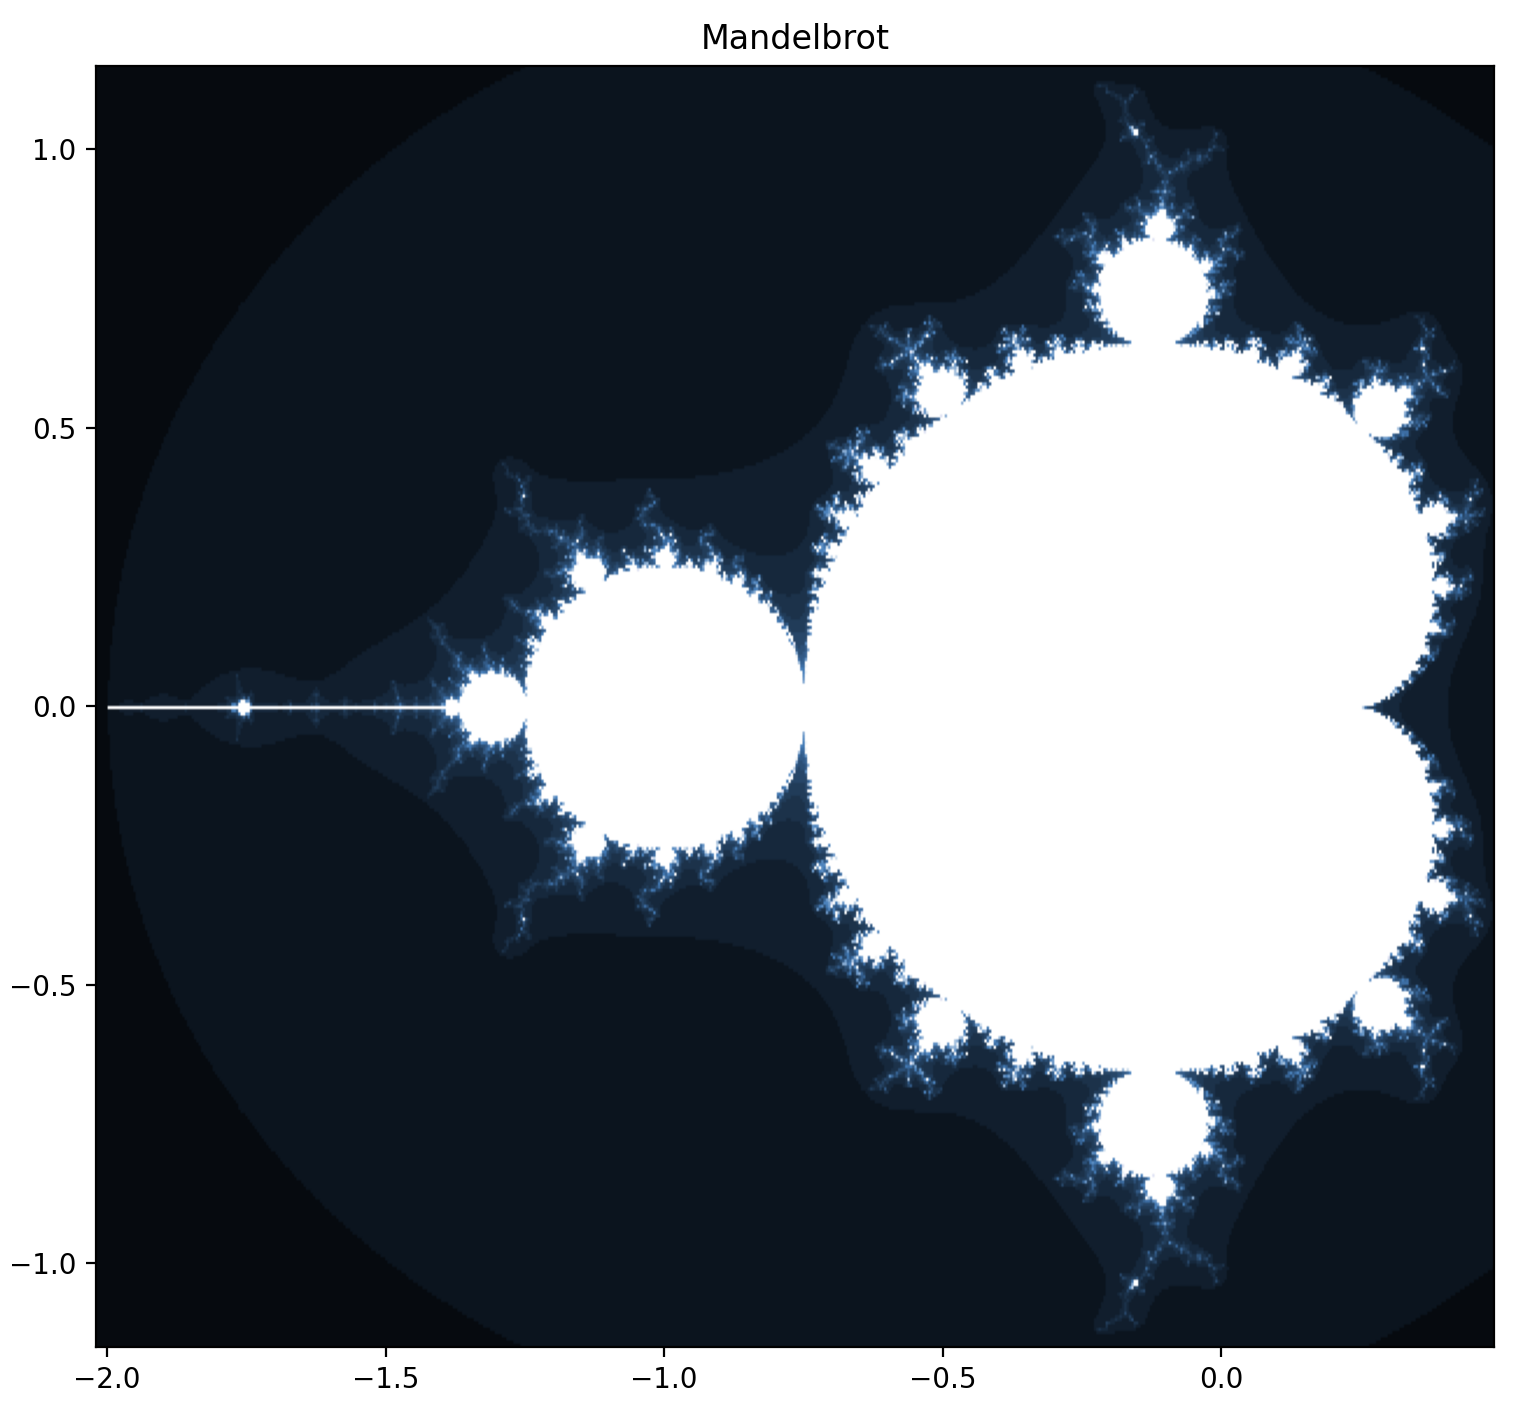
\includegraphics[width=.8\textwidth]{pictures/part_1/mandelbrot_set_1.png}
        \caption{Representation of Mandelbrot set with maximal iteration set at 100. Complex point part of the set are in white. The first bulb (period 2) is visible as a disk centered on centered on $c = -1$ and tangent to the left of main cardioid (period 1) in $c=-\frac{3}{4}$.}
        \label{fig:mandelbrot_set}
    \end{figure}

    \begin{figure}[h]
        \begin{subfigure}[t]{.48\linewidth}
            \centering
            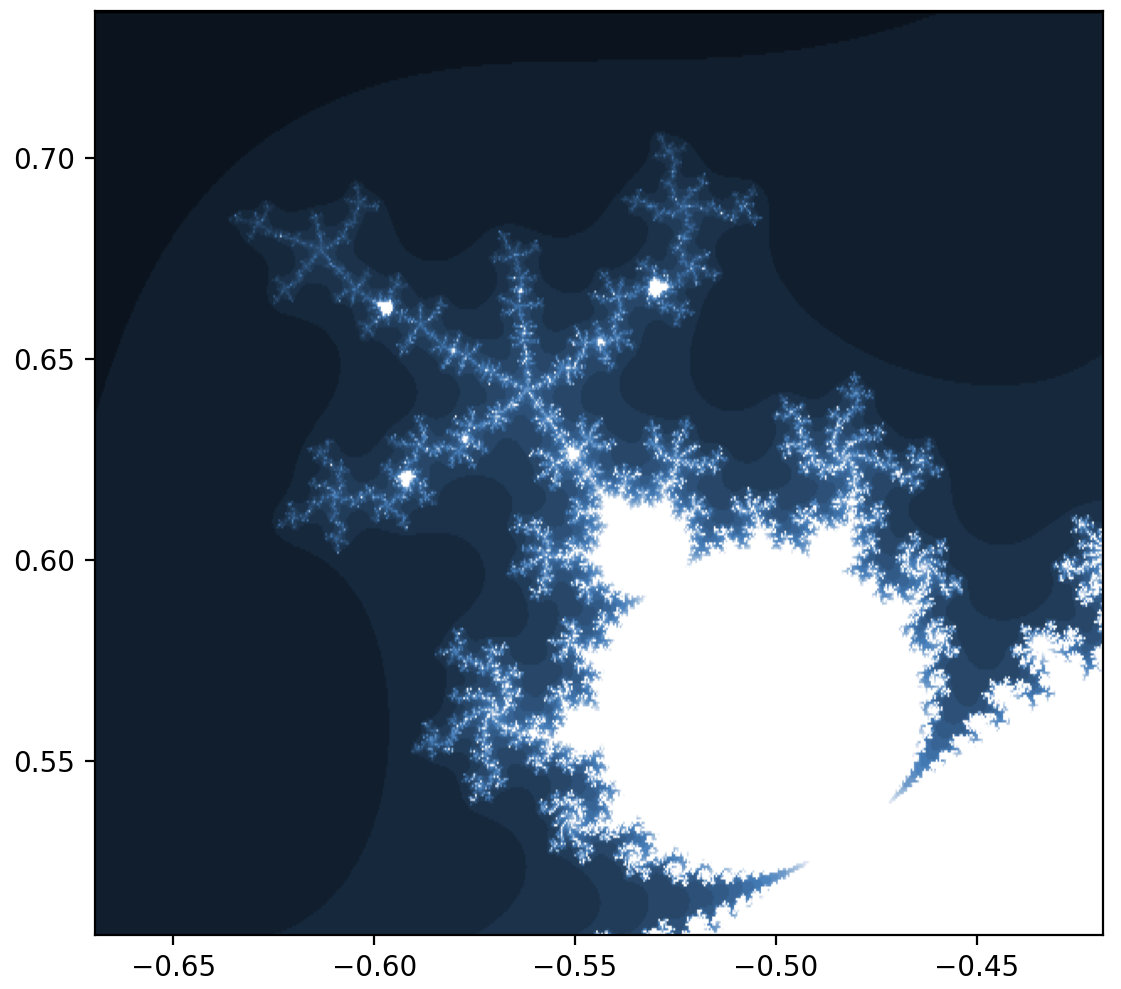
\includegraphics[width=.9\textwidth]{pictures/part_1/mandelbrot_set_bulbs_10_5.png}
            \caption{Period 5 and period 10 bulb. Period of the bulbs can be easily determined by the number of \emph{antenna} they have}
            \label{fig:mandelbrot_set_bulb_5_10}
        \end{subfigure}
        \begin{subfigure}[t]{.48\linewidth}
            \centering
            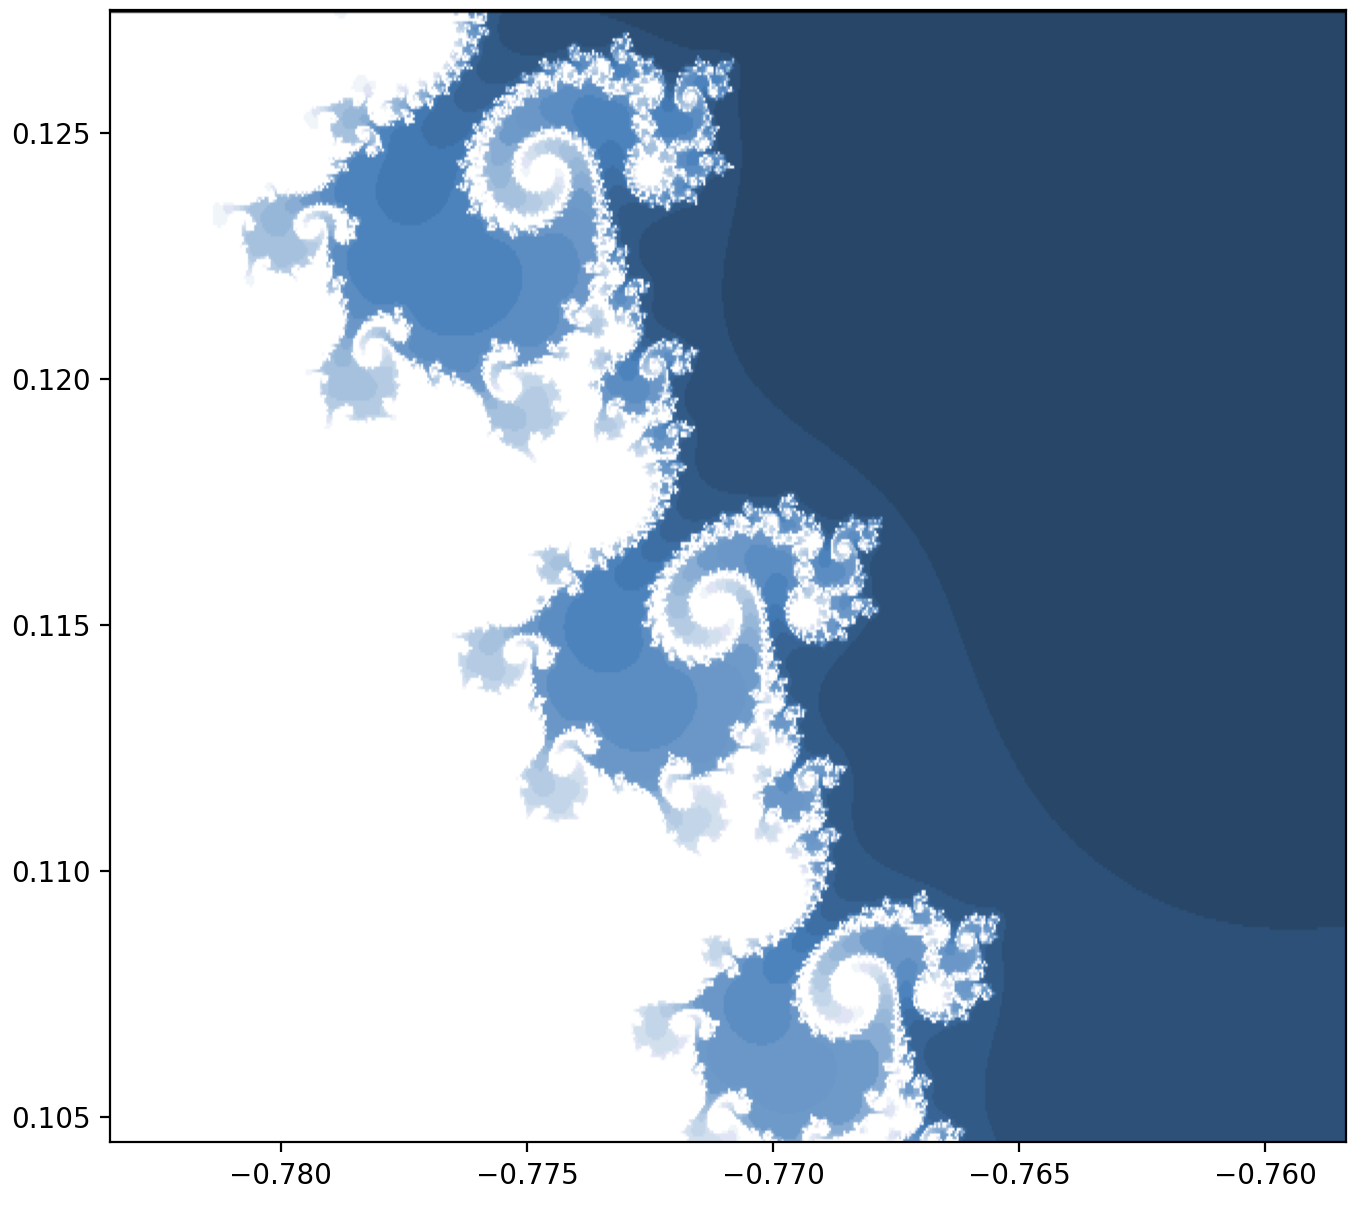
\includegraphics[width=.9\textwidth]{pictures/part_1/mandelbrot_set_spiral.png}
            \caption{Double spiral are visible in all regions close to tangent points}
            \label{fig:mandelbrot_double_spiral_seahorse_valley}
        \end{subfigure}
        \caption{Visualisation of structures in Mandelbrot set}
        \label{fig:mandelbrot_set_bulbs}
    \end{figure}

    \subsubsection*{Convergence in Complex Plane}

    While studying the properties of Mandelbrot set and its graphic representation, we investigated the convergence of the complex numbers within the recurrence sequence.\\ To our surprise, we learn that points in different regions of the complex plane of the Mandelbrot set will not converge in the same way. As observed in Appendix \ref{appendix:convergence_c} Figure \ref{fig:complex_points_convergence_fast} and \ref{fig:complex_points_convergence_slow}, as we get closer to the boundaries of Mandelbrot set, the points from the complex plan will converge more slowly to an attracting fixed point. More over, we figured that complex numbers might not converge to a unique attracting point (See Appendix \ref{appendix:convergence_c} Figure \ref{fig:complex_points_convergence_multiple}), while they could still remain within the Mandelbrot set. We can link this latest observation to the escape criterion property: the Mandebrot set is contained in a circle of radius 2 centered to the origin, thus allowing convergence to multiples fixed points within this circle.

    \subsection{Estimation by Monte-Carlo approach}
    \label{section:part_2_monte_carlo}

    \subsubsection*{Implementation}

    The package \emph{numpy} we use in our implementation of the Monte-carlo algorithm provides a continuous uniform random number generator good enough for our approximation. While we can note that the possible generated random values remains bounded to double precision approximation (\emph{float64}), it goes far beyond the computing power available and so is not an issue in the approximation of the mean area.\\
    Thus, the transcription from the Monte-Carlo method theory (See Section \ref{subsection:monte_carlo_theory}) into our numerical algorithm highlighted the main two parameters we will have to study: number of samples in the complex plan and maximal number of iterations of the recursive sequence.\\

    \subsubsection*{Convergence of Monte-Carlo algorithm}

    \textbf{Influence of maximal number of iterations}\\

    From the former research, we know that the theoretical convergence $\frac{1}{\sqrt{S}}$ of Monte-Carlo algorithm depends on the number of samples $S$. However, as we need to get a proper estimation of the area of the Mandelbrot set, we decided in the first instance to focus our attention on the maximal number of iterations to consider: with a maximal number of iterations too small most points from the complex plan will be considered as part of the Mandelbrot set; while a value too high will results in a waste of computing resources.\\
    To investigate the number of iterations required for a good estimate, we fixed a number of samples at $S = 5000$ (Not fully arbitrary considering the theoretical convergence of $\frac{1}{\sqrt{S}} \approx 0.014$), and run $50$ simulations to get a more accurate approximation of the relative error:

    \begin{equation}
        \epsilon = \frac{|A_{js} - A_m|}{|A_m|} \approx \frac{|A_{js} - A_{is}|}{|A_{is}|}
    \end{equation}

    \begin{figure}[h]
        \centering
        \begin{subfigure}[t]{.48\linewidth}
            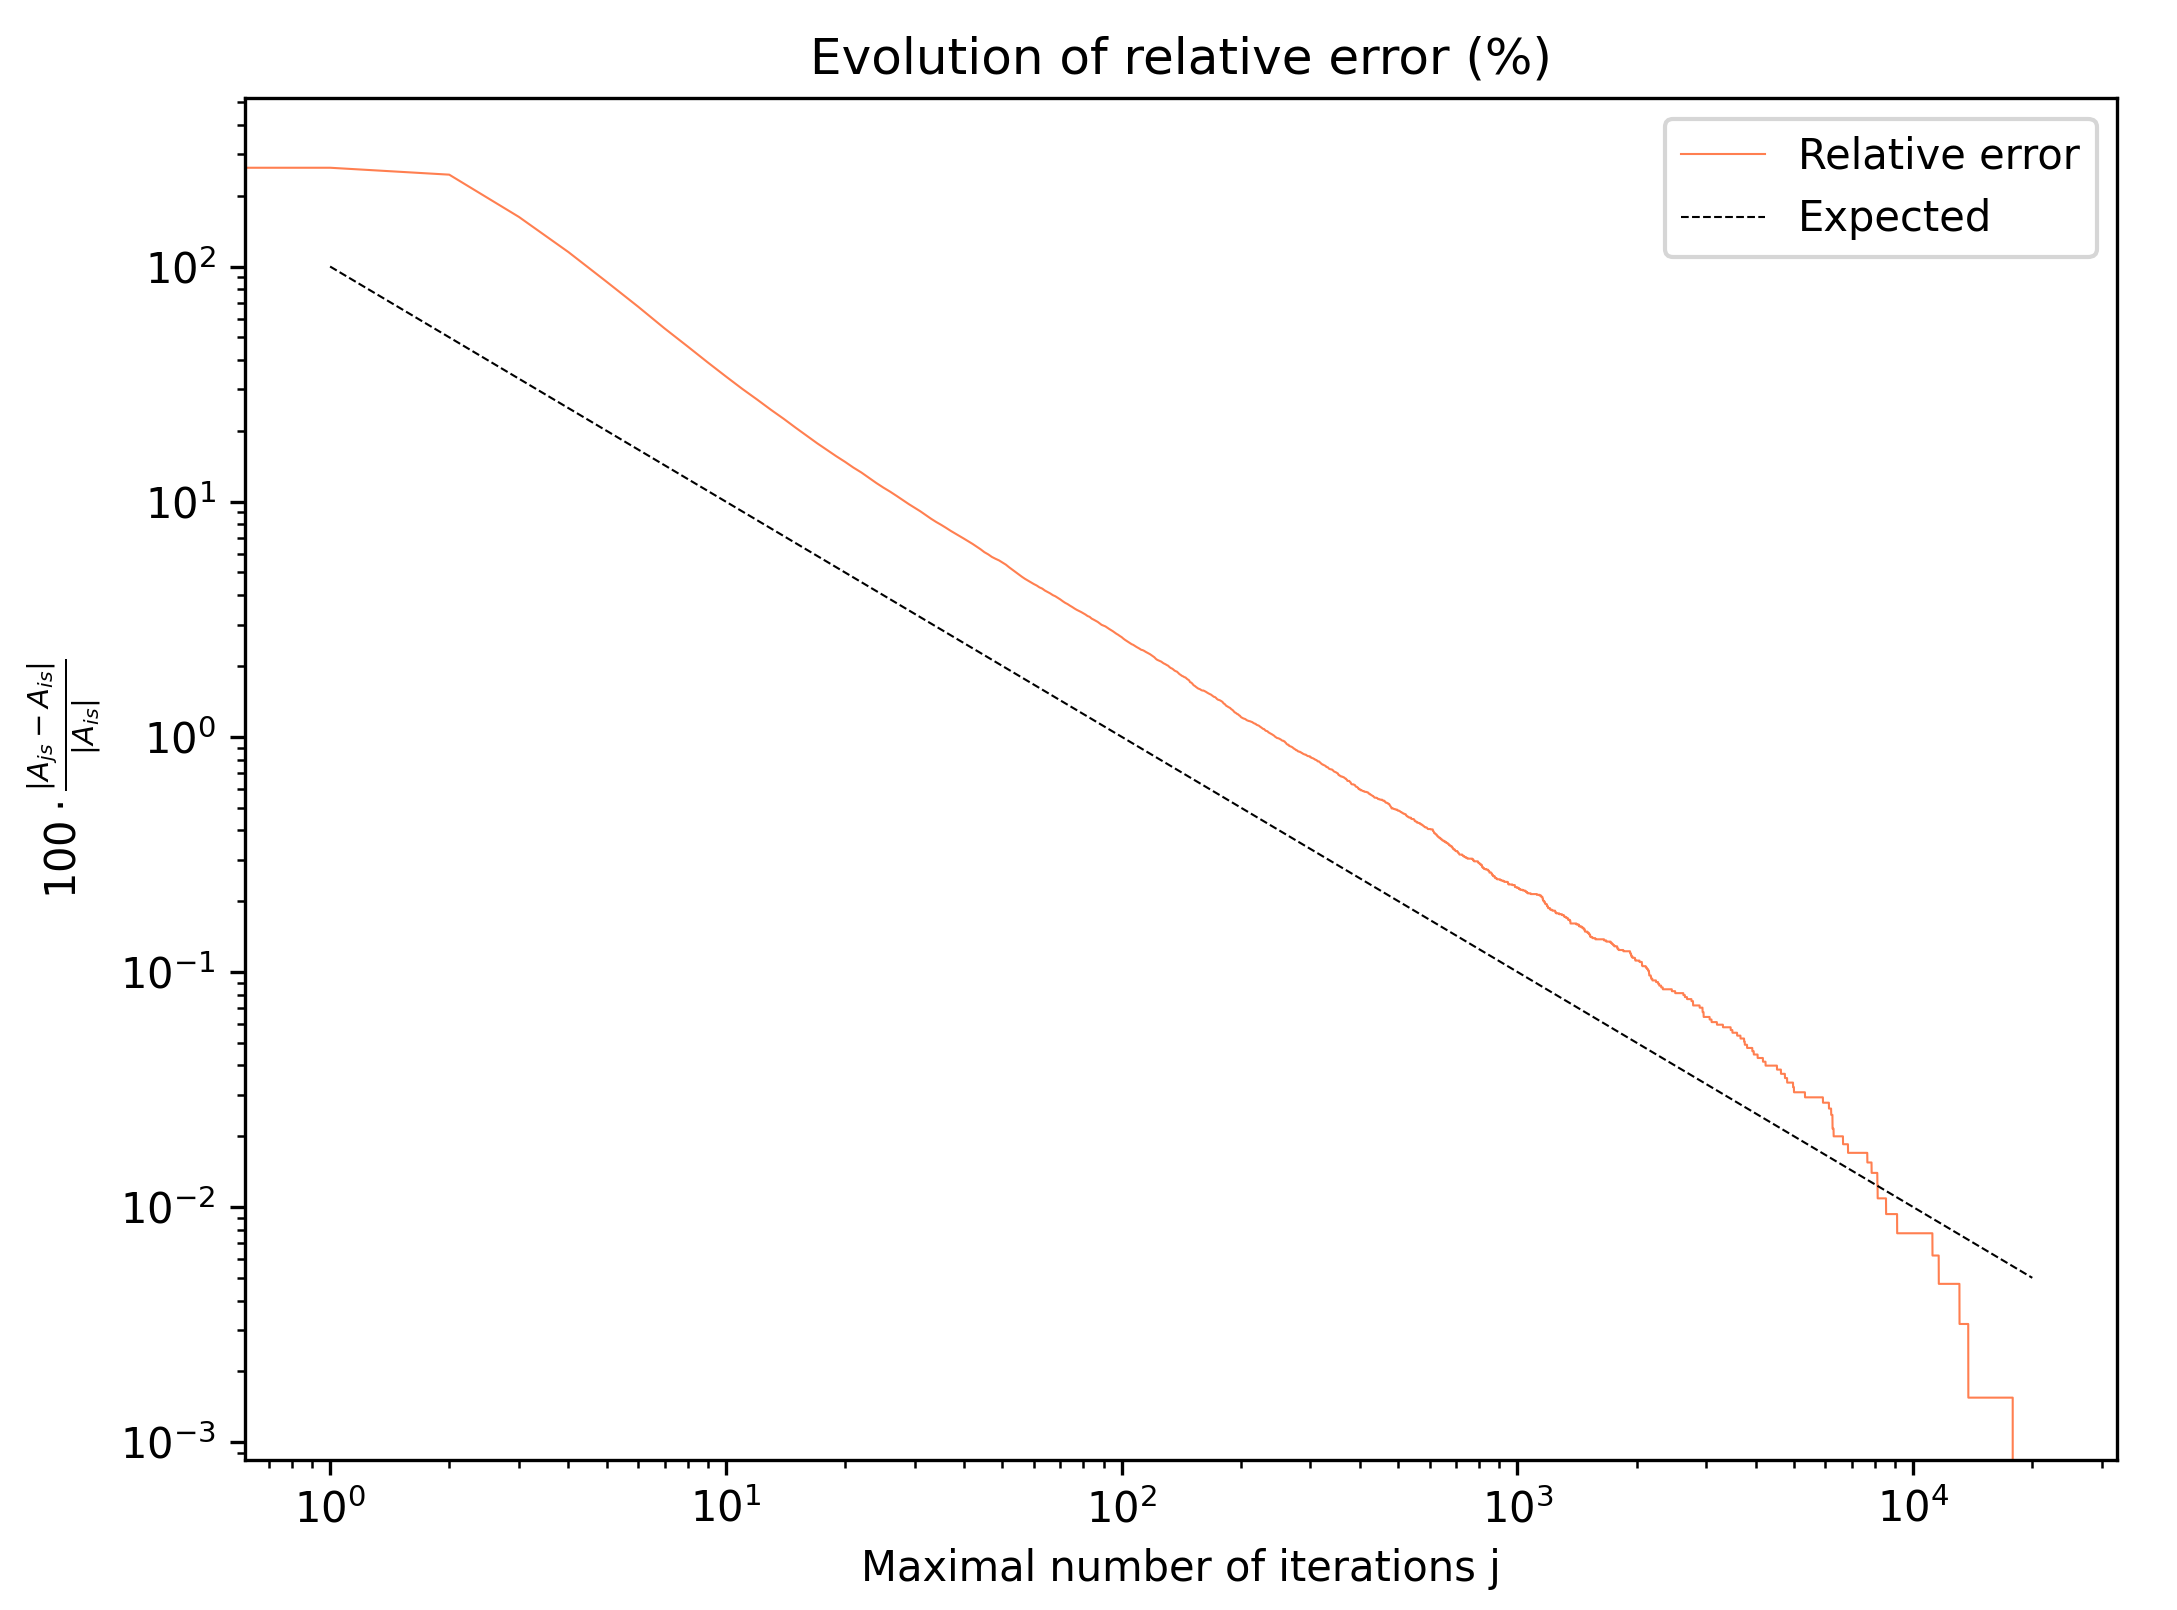
\includegraphics[width=\textwidth]{pictures/part_2/maximal_number_iteration_convergence.png}
            \caption{Evolution of relative error using pure random sampling, by maximal number of iteration up to $20,000$ and number of samples equal to $5000$ }
            \label{fig:maximal_iteration_relative_error}
        \end{subfigure}
        \begin{subfigure}[t]{.48\linewidth}
            \centering
            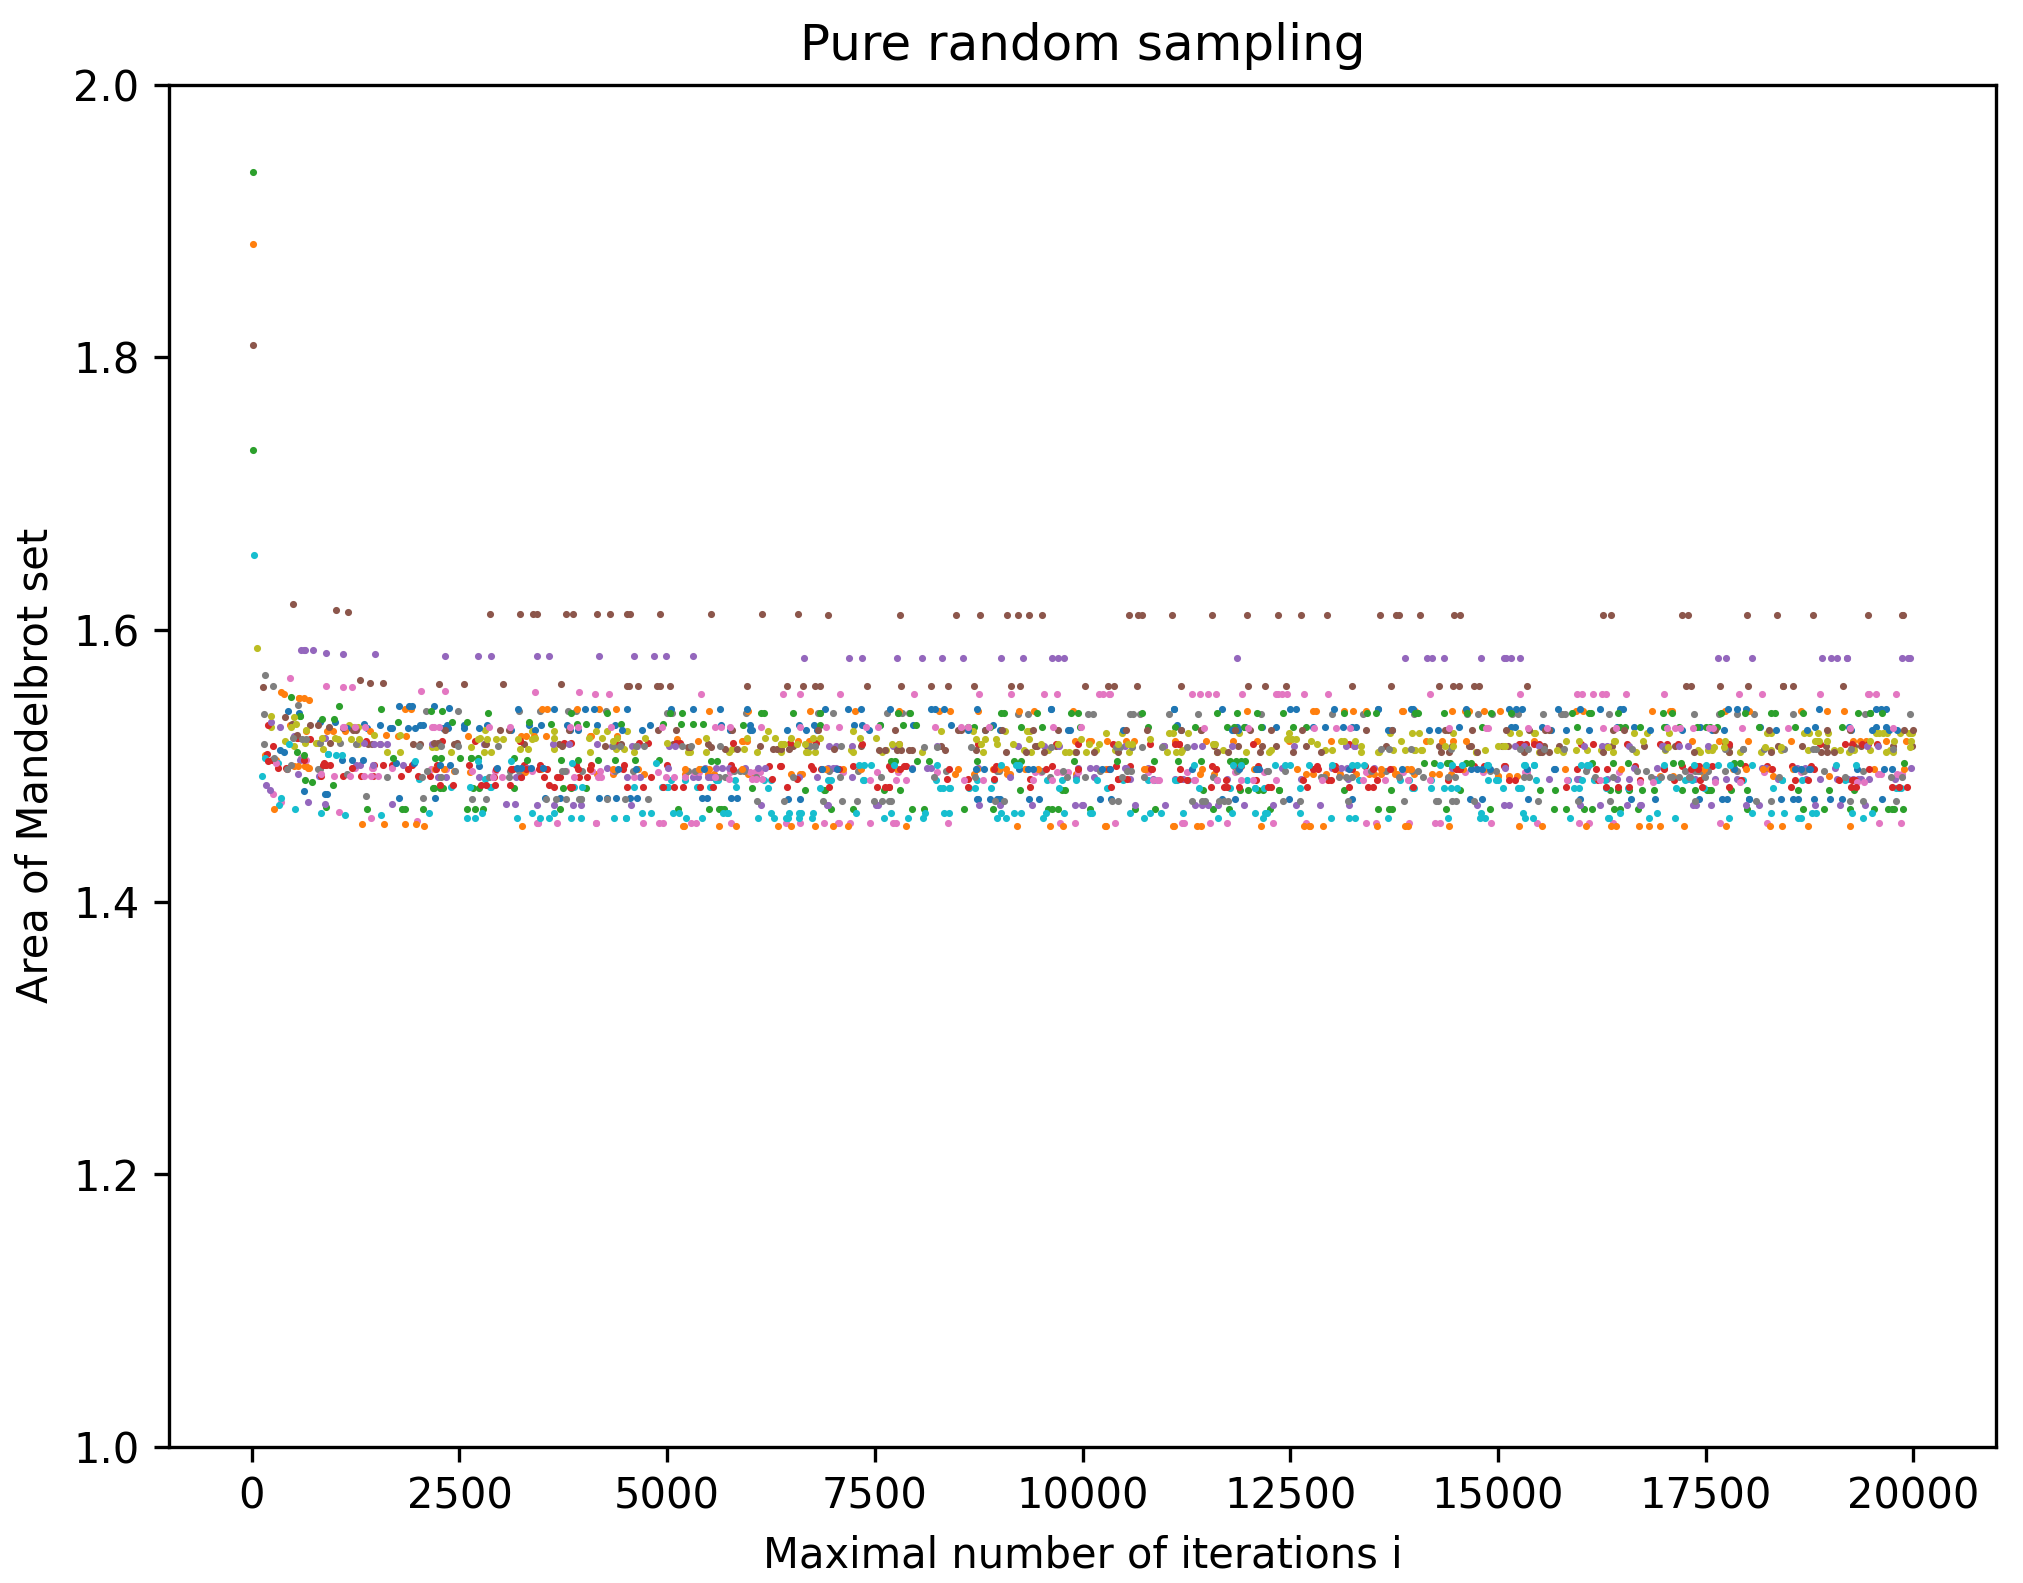
\includegraphics[width=\textwidth]{pictures/part_2/maximal_number_iteration_area_50_simulations.png}
            \caption{Evolution of Mandelbrot set area based on maximal number of iteration up to $20,000$}
            \label{fig:maximal_iteration_area_evolution}
        \end{subfigure}

        \caption{Impact of maximal number of iteration over Monte-Carlo approach results}
        \label{fig:maximal_iteration}
    \end{figure}


    The Figure \ref{fig:maximal_iteration_relative_error} visualizes a convergence rate close to $\frac{1}{I}$ (with $I$ maximal number of iterations). We highlight the fact that the estimated relative error is an approximation itself (while acceptable), given that we used the estimated area $A_{is}$ (Which in the context of this Figure was estimated at $A_{is} \approx 1.503035$), instead of a 'true' accurate area estimate $A_m$ of Mandelbrot set (with the most accurate approximation as of current research is $\approx 1.50659177$). The Figure \ref{fig:maximal_iteration_area_evolution} also bolstered the fact that the area sample mean doesn't deviate significantly after $1000$ iterations. Therefore, it appears that setting a maximal number of iterations around $1000$ would provide the level of error acceptable for the purposes of this report.\\

    \textbf{Influence of sample set size}\\
    As a next step we want to confirm the expected Monte-Carlo convergence rate $\frac{1}{\sqrt{S}}$, and come to a first estimation of the Mandelbrot set area.

    \begin{equation}
        \epsilon = \frac{|A_{it} - A_m|}{|A_m|} \approx \frac{|A_{it} - A_{is}|}{|A_{is}|}
        \label{eq:samples_relative_error}
    \end{equation}


    \begin{figure}[h]
        \centering
        \begin{subfigure}[t]{.48\linewidth}
            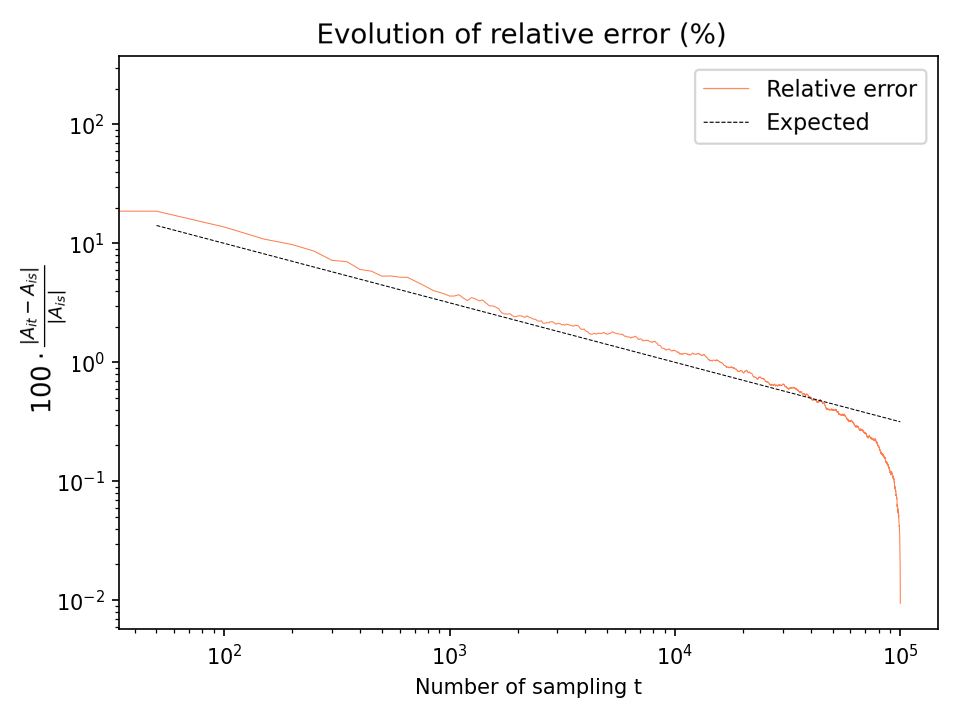
\includegraphics[width=\textwidth]{pictures/part_2/number_samples_convergence.png}
            \caption{Evolution of relative error using pure random sampling, by number of samples up to $100000$ with maximal number of iteration set at 1000.}
            \label{fig:samples_relative_error}
        \end{subfigure}
        \begin{subfigure}[t]{.47\linewidth}
            \centering
            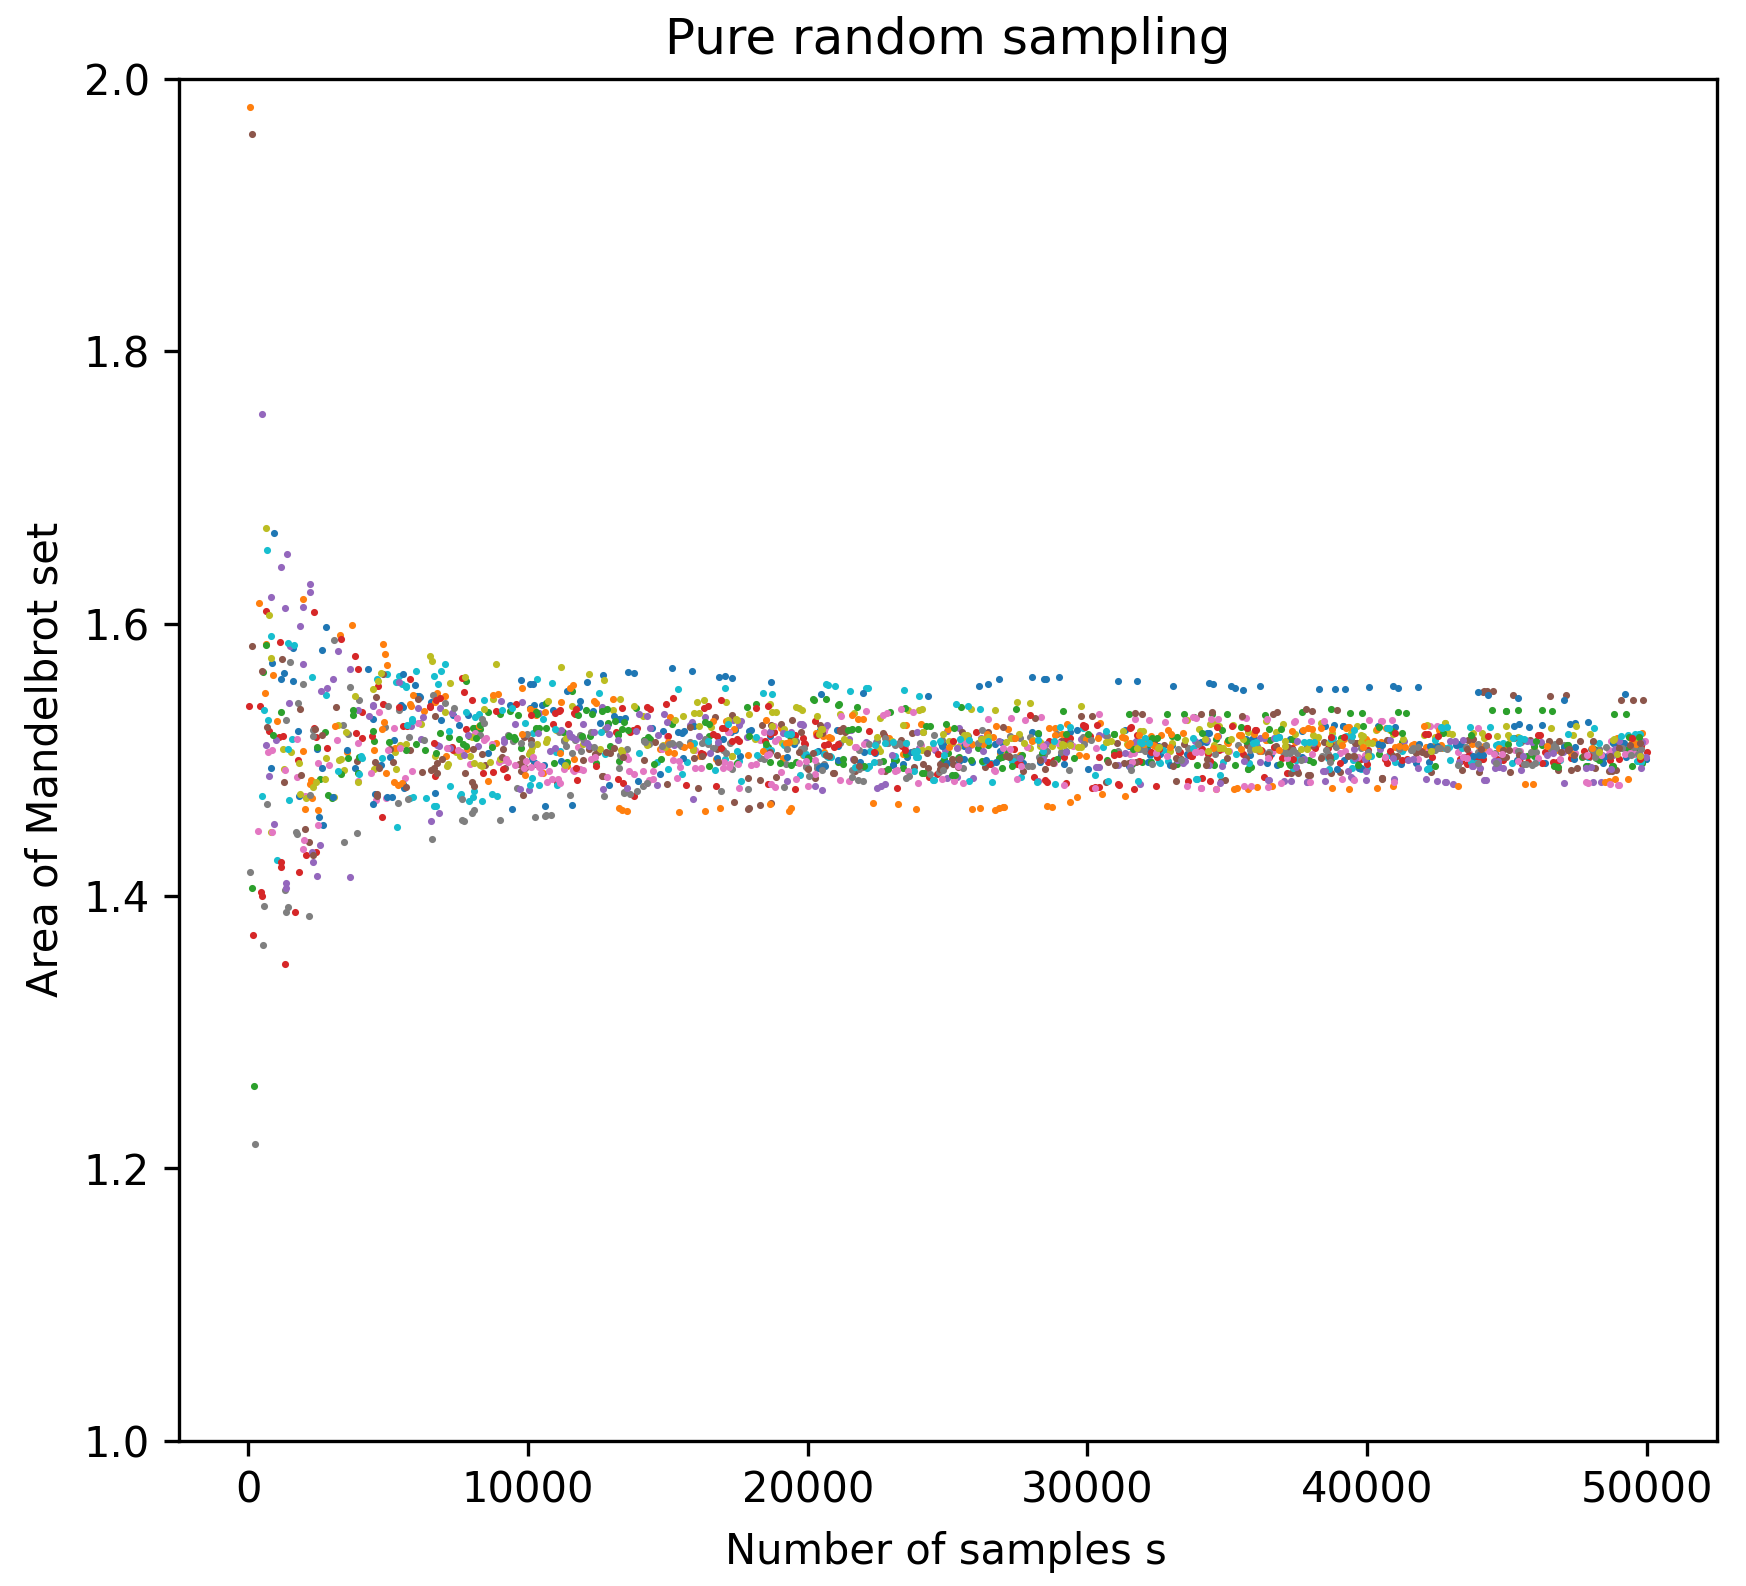
\includegraphics[width=\textwidth]{pictures/part_2/number_samples_area_50_simulations.png}
            \caption{Evolution of Mandelbrot set area based on maximal number of iteration}
            \label{fig:samples_area_evolution}
        \end{subfigure}

        \caption{Impact of maximal number of iteration over Monte-Carlo approach results}
        \label{fig:samples}
    \end{figure}

    We ran 50 simulations to visualize the relative error (See Eq \ref{eq:samples_relative_error}) as well as the convergence to the estimated area.\\
    On the Figure \ref{fig:samples_relative_error} we can observe the evolution of the relative error by number of samples up to $100,000$ with a maximal number of iteration set at $1000$. As expected (See Section \ref{subsection:monte_carlo_theory} on Monte-Carlo method) the simulations shows that Monte-Carlo approach using pure random sampling will have a convergence rate close to $\frac{1}{\sqrt{S}}$ (black line). We reiterate that the last part of the curve should be dismissed: our implementation generates a set of sample points, then computes the relative error for all of these samplings, therefore, the last values are close to $A_is$ the last expected value computed and so the error tends to 0.\\
    In addition to the Figure \ref{fig:samples_relative_error} which shows a small relative error; the Figure \ref{fig:samples_area_evolution} also confirm the fact that from $5000$ samples the average area estimated does not change significantly, and so for the following experiments, with our computing power available, we can consider this number of samples.\\

    From these initial experiments, we can conclude on the efficiency of Monte-Carlo approach to estimates mean values. However, we could as well highlights the fact that we remains limited on computing power and this remains quite a slow solution to get accurate estimation beyond $10^{-3}$ precision.
    Therefore, the logical next step consists in investigating methods which would enable us to speed up the convergence to an accurate approximation of the Mandelbrot set area, among these techniques we think mainly about variance reduction, which make good usage of new sampling techniques.


    \subsection{Experiments with various sampling methods}

    In the previous part of the report we have focused on pure random sampling, where every point is chosen randomly and entirely by chance, such that each point in the complex plane has the same probability of being chosen at any stage during the sampling process, and each subset of j points has the same probability of being chosen for the sample as any other subset of j points. Instead, we will now explore stratified sampling methods, those methods which are concerned with splitting our complex plane into sub-domains.

    First, we will compare the statistical properties of our area estimates using LHS and Orthogonal sampling given a fixed number of sampling points, a fixed number of iterations and a fixed number of simulations. Then, we will implement the 'when to stop algorithm' and investigate the convergence properties of the stratified sampling methods.

    The first experiment, run with a fixed number of simulations and thus a fixed number of area estimates for each method, aims to investigate if our alternative sampling methods really reduce output sample variance for a fixed number of simulations over the pure random method. For each sampling method we estimate the area of the set 50 times and make estimates for the summary statistics of each sample. The area of our Mandelbrot set is estimated over the complex plane: real part (- 2.02, 0.49) and imaginary part (-1.15, 1.15). Our maximum iterations is set as 800. For each method we only sample 2500 points in the complex plane. This might not be the optimum sampling volume for estimation accuracy but given our compute power constraints, it is appropriate. Using a smaller sampling volume will also accentuate the variance reduction and accuracy increases we will (hopefully) achieve with the stratified sampling methods. For each method we will investigate the sample mean, sample variance and the confidence interval.

    \begin{table}[h!]
        \centering
        \begin{tabular}{|c | c | c | c|}
            \hline
            Sampling Method & Sample Mean & Sample Variance & Conf. Interval (p = 0.95) \\
            \hline\hline
            Pure Random & 1.5220 & 2.46 x $10^{-3}$ & [1.50827, 1.53580] \\
            Latin Hypercube & 1.5142 & 8.39 x $10^{-4}$ & [1.50625, 1.52231] \\
            Orthogonal Sampling & 1.5082 & 7.58 x $10^{-5}$ & [1.50586, 1.51069] \\
            \hline
        \end{tabular}
        \caption{}
        \label{Table:q3e1}
    \end{table}

    The sampling variance results are shown in Table~\ref{Table:q3e1}. LHS provides lower variance estimates than pure random and Orthogonal Sampling provides the estimate with the lowest sample variance. Because the range of our confidence intervals depends directly on the sample standard deviation, it is unsurprising that the confidence interval ranges in LHS and orthogonal are smaller than those from pure random sampling. For each method above, we can interpret the confidence interval as the following: if this test was repeated again numerous times, the fraction of calculated confidence intervals (which would differ for each sample) that encompass the true area value would tend toward 95\%. The range of the confidence intervals is decreasing in the methods, it is fair to say that given a fixed confidence interval, we can be more sure of the accuracy of an estimate obtained from Orthogonal Sampling than we can from an estimate obtained using Latin Hypercube Sampling.

    The second experiment involves setting some fixed level of sample standard deviation we wish to achieve with our methods, then running repeated simulations with each method until we achieve the desired target. Again, our maximum iterations = 800 and on each simulation run we only sample 2500 points. We set a minimum number of simulations = 50, so for very low variance methods we still achieve a sample size large enough to draw conclusions from. We will perform the experiment according to the following algorithm:
    \begin{enumerate}
        \item Choose some starting standard deviation: $d = 0.008$
        \item Generate/collect at least k = 50 samples
        \item Continue collection samples, until $\frac{S}{\sqrt{k}} < d$
        \item Estimate of $\theta$ is then given as $\overline{X} = \sum_{i} \frac{X_i}{k} $
    \end{enumerate}

    \begin{table}[h!]
        \centering
        \begin{tabular}{|c | c | c | c|}
            \hline
            Sampling Method & Simulations & Sample Mean & Conf. Interval (p = 0.95) \\
            \hline\hline
            Pure Random & 149 & 1.5093 & [1.5053, 1.5133] \\
            Latin Hypercube & 80 & 1.5114 & [1.5074, 1.5153] \\
            Orthogonal Sampling & 50 & 1.5105 & [1.5093, 1.5117] \\
            \hline
        \end{tabular}
        \caption{}
        \label{Table:q3e2}
    \end{table}

    The results are shown in Table~\ref{Table:q3e2}. As expected, given some fixed standard deviation to achieve, our stratified methods of sampling converge more quickly on this value than the pure random method. Our orthogonal sampling simulation achieved the required standard deviation extremely quickly; it stopped at the minimum simulations condition, it is likely that the method achieved the required estimate variance even earlier in the experiment. Note that the stochastic simulation we deal with in this paper is not particularly complex and thus we can quite easily compute 100s of simulation results on a normal laptop. The real power of variance reduction techniques is seen in domains where a single simulation result can take many compute-days to obtain. In these cases reducing the number of simulation runs required to obtain an accurate result can save researchers substantial resources.

    We now investigate the convergence behaviour of our area estimation as we vary maximum amount of iterations of the quadratic recurrence equation, for each of our sampling methods. We will compare the behaviour of the stratified methods to the convergence dynamics of pure random sampling we saw previously. In this experiment we draw 10,000 samples with each method, enough that the number of samples drawn will not be the limiting factor of the convergence of our variance. Figure~\ref{fig:stratified_it} demonstrates that increasing iterations has little effect on the convergence of the variance of our estimate. Each method appears to have some level of variance around which it oscillates, independent of the maximum number of iterations.   Figure~\ref{fig:stratified_var} shows the results of a similar experiment, with the estimate variance being shown as a function of sampling volume and the number of iterations of the recurrence equation fixed at 800. The 3 sampling methods have decreasing variance, but at a similar gradient for each method. It is clear that orthogonal sampling has a substantially lower estimate variance for any given level of sampling.

    \begin{figure}[!tbp]
        \centering
        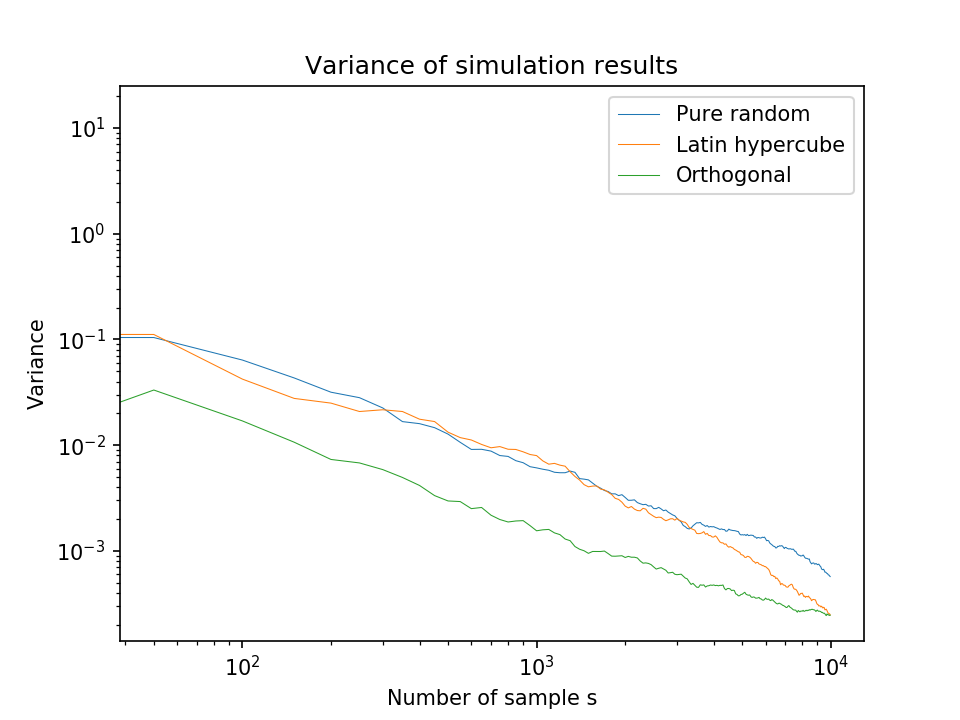
\includegraphics[width=0.75\textwidth]{pictures/part_3/q_3_variance.png}
        \caption{Sampling Variance Convergence}
        \label{fig:stratified_var}
    \end{figure}

    \begin{figure}[!tbp]
        \centering
        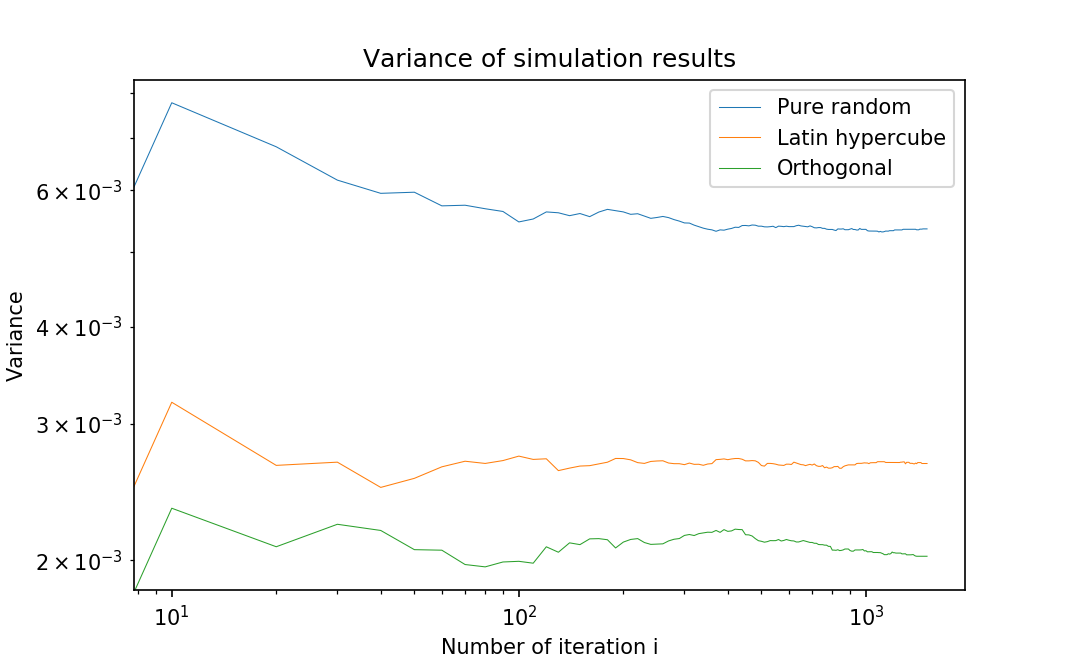
\includegraphics[width=0.75\textwidth]{pictures/part_3/q_3_iterations.png}
        \caption{Convergence as a function of Maximum Iterations of the Quadratic Recurrence Equation}
        \label{fig:stratified_it}
    \end{figure}

    \subsection{Improvement of Monte-Carlo approach convergence rate}

    To further improve the convergence rate of our simulation, we have chosen to implement the Randomised Quasi-Monte Carlo Method, which uses randomly shifted low-discrepancy sequences as described in the 'Method' section above. Broadly, we can think of the discrepancy as a metric describing the highest and lowest density of points in a sequence. High discrepancy means that there are either a large areas of empty space, or that there are area with an unusually high density of samples. Low discrepancy means that there are neither, and that your points are distributed reasonably evenly. Figure~\ref{fig:halton_sample} shows a sample of grid points generated using this method, note the reasonably consistent sampling density across the entire grid plane. In contrast,  Figure~\ref{fig:pure_random_sample} shows a plane sampled with points purely randomly. With a pure random approach, we see there are \emph{clumps} of points generated very close together and some areas of the plane with very few sampled points. This demonstrates that randomly shifted Halton Sequences allow us to sample our complex plane in a manner which has a discrepancy lower than that which pure sampling alone would allow.


    \begin{figure}[!tbp]
        \centering
        \begin{minipage}[b]{0.45\textwidth}
            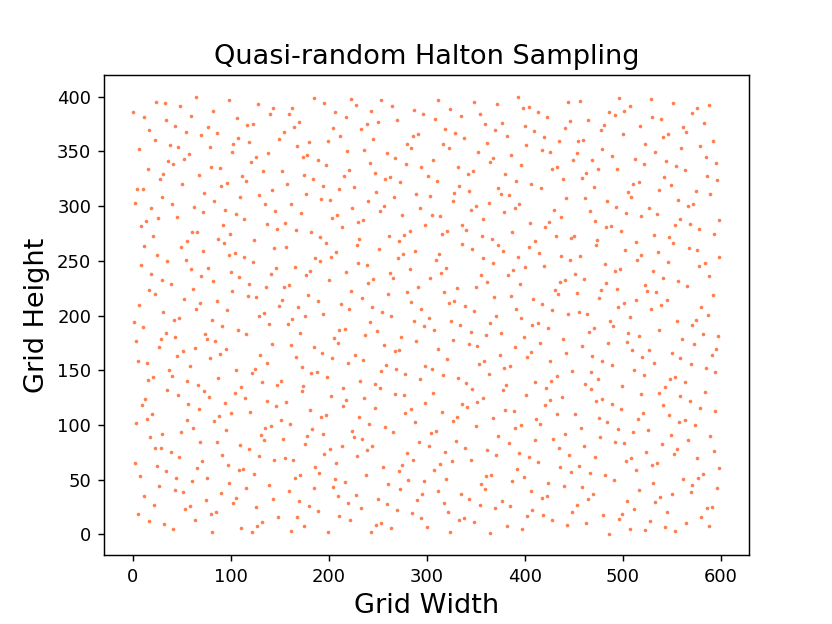
\includegraphics[width=\textwidth]{pictures/part_4/halton.png}
            \caption{Example Sample, Randomised Low Discrepancy Sequence}
            \label{fig:halton_sample}
        \end{minipage}
        \hfill
        \begin{minipage}[b]{0.45\textwidth}
            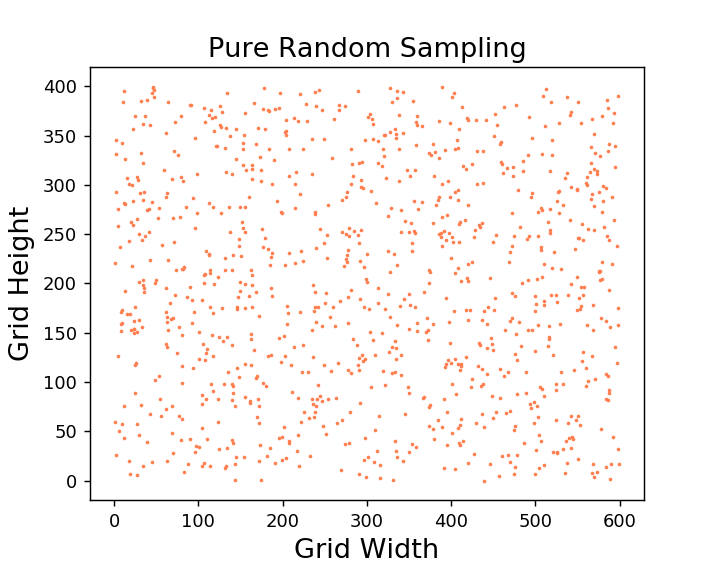
\includegraphics[width=\textwidth]{pictures/part_4/pure_rand.png}
            \caption{Example Sample, Pure Random}
            \label{fig:pure_random_sample}
        \end{minipage}
    \end{figure}


    \begin{table}[h!]
        \centering
        \begin{tabular}{|c | c | c | c|}
            \hline
            Sampling Method & Sample Mean & Sample Variance & Conf. Interval (p = 0.95) \\
            \hline\hline
            Orthogonal & 1.5102 & $2.5103 \times 10^{-5}$ & [1.5087, 1.5115] \\
            Randomised Halton Sequence & 1.5056 & $7.9266 \times 10^{-6}$ & [1.5048, 1.5064] \\
            \hline
        \end{tabular}
        \caption{}
        \label{Table:q4_fixedsim}
    \end{table}

    Table~\ref{Table:q4_fixedsim} contains the summary statistics for an experiment run with our Randomised Quasi-monte carlo method and our best implementation of the monte carlo method with stratified sampling. We run 50 simulations and in each run, we sample 10,000 points in the complex plane. We consider a point in the complex plane to be part of the Mandelbrot set if it has not met the escape criteria after 800 iterations of the quadratic recurrence equation. Our Halton sequence leads to a sample variance on an order of magnitude lower than that of the orthogonal sampling method, suggesting that randomised quasi-monte carlo does, on average, lead to a lower more accurate estimation of the area given finite compute power. This reduced sampling variance gives us a confidence interval with a tighter range.

    We now perform a similar experiment, but this time use the 'when to stop' algorithm to investigate convergence upon a target standard deviation of 0.0025, and observe how long convergence takes for each method. Again, our escape criteria is set to 800 iterations of the quadratic recurrence equation and 2500 points are sampled in each run. We repeat the 'when to stop' process 30 times for each method and then take the sample mean of the convergence times. The results are shown in Table~\ref{Table:q4conv}.

    \begin{table}[h!]
        \centering
        \begin{tabular}{|c | c | c | c|}
            \hline
            Sampling Method & Mean Simulations before Convergence & Simulations Sample Variance\\
            \hline\hline
            Orthogonal & 352 & 7493 \\
            Randomised Halton Sequence & 71.7 & 156.4 \\
            \hline
        \end{tabular}
        \caption{}
        \label{Table:q4conv}
    \end{table}

    To test whether there is a significant difference between the number of simulations required for convergence between the two methods, we can use the two-sample parametric Welch test. Welch's test is used to determine if two population means are equal. Welch's test is an adaption of the student's t-test, except that it is more reliable when the two samples have unequal variances and/or unequal samples sizes. We have chosen the Welch's test because Table~\ref{Table:q4conv} shows that the iterations values obtained for our two methods have a large difference in sample variance. Although the test is designed for unequal sample distribution variance, the assumption of sample distribution normality is maintained.

    We can take our null hypothesis to be that the two population means are equal, that is, there is no difference in the mean number of simulations required to converge on our target standard deviation. Our alternative hypothesis is then that there is a statistically significant difference in the mean number of simulations required to converge on our target standard deviation. We set our confidence level to be 0.95. Our test statistic given as:

    \begin{equation}
        t = \frac{\overline{X}_1 - \overline{X}_2}{\sqrt{\frac{s_1^2}{N_1} + \frac{s_2^2}{N_2}}} = 17.56
    \end{equation}

    Where $\overline{X}_1$ is the mean number of simulations before convergence under Orthogonal, and $\overline{X}_2$ is the equivalent under Halton Sampling. $s_1$ and $s_2$ denote the sample standard deviation for our simulation values for each method. $N_1$ and $N_2$ denotes the number of data points, which in our case is the same for each of our two samples. We computed our t statistic with the Scipy.stats.ttest\_ind() function. The critical value to which we compare our test statistic will be given by $T^{-1}_{f}(\frac{p + 1}{2})$ where f is the degrees of freedom as described by the Welch–Satterthwaite equation. The absolute value of our test statistic (17.56) is clearly far larger than the critical value and so we can reject our null hypothesis that the two mean simulation values are the same. It seems that Randomised low discrepancy sequences do reduce the amount of simulations required to obtain a particular standard deviation, at least within the experimental frame defined here.\\


    \begin{figure}[!tbp]
        \centering
        \begin{minipage}[b]{0.75\textwidth}
            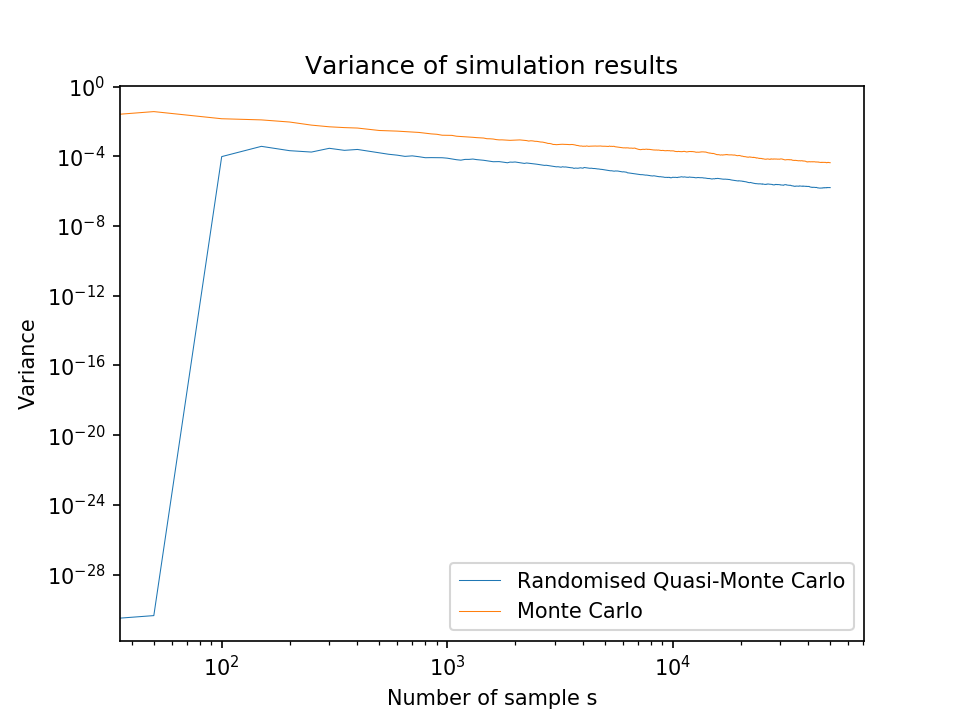
\includegraphics[width=\textwidth]{pictures/part_4/sampling_q4.png}
            \caption{Convergence behaviour as a Function of Sampling Volume}
            \label{fig:q4sampling}
        \end{minipage}
    \end{figure}

    \begin{figure}[!tbp]
        \centering
        \begin{minipage}[b]{0.75\textwidth}
            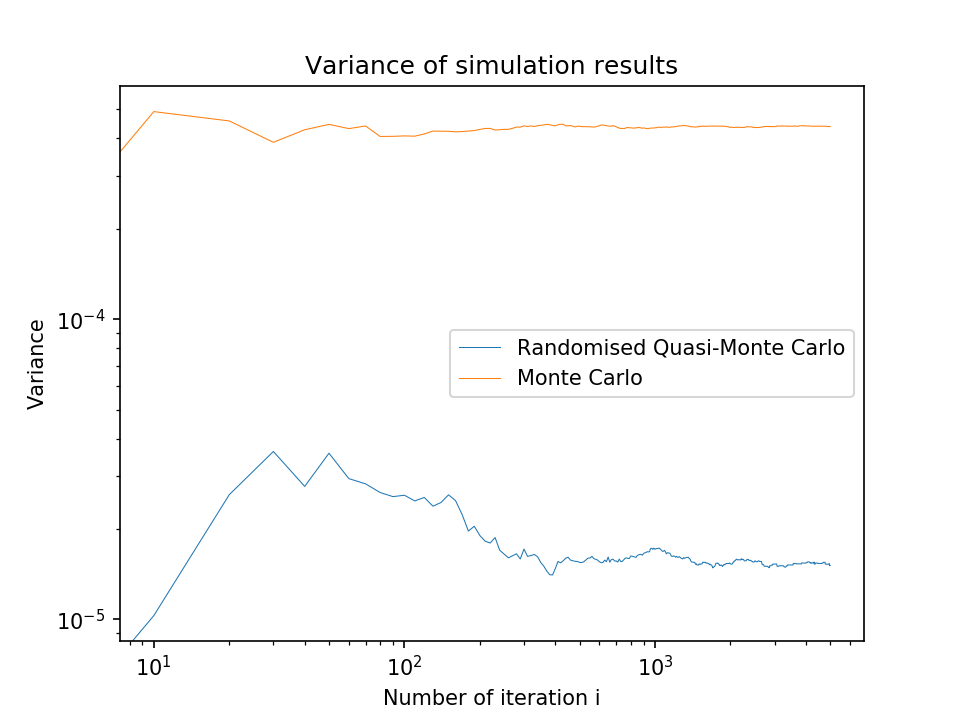
\includegraphics[width=\textwidth]{pictures/part_4/iterations_q4.png}
            \caption{Convergence behaviour as a Function of Iterations}
            \label{fig:q4iter}
        \end{minipage}
    \end{figure}

    Figure~\ref{fig:q4sampling} shows how the variance of our area estimates converge as we increase the number of points sampled in the complex plane per simulation. note that for very low sampling volume, the Halton method has extremely low variance. This is due to the semi-deterministic nature of Halton sampling and we believe that the variance estimation at low sampling volume is quite inaccurate. Note that after approximately $10^2$ samples, both methods converge at approximately the same rate, however Halton sampling has a lower absolute value of variance for any given number of samples. Figure~\ref{fig:q4iter} shows how the area estimates converge as we increase the number of iterations of the quadratic recurrence equation. While the quasi-MC has a lower absolute value of variance, it seems that iterations play less of a role in convergence behaviour for both methods than sampling volume. For the standard MC, variance is relatively constant with the number of iterations. For quasi-MC, we see slightly higher variance before $50^2$ iterations, but relatively stable behaviour after.

    \section*{Conclusion}
    Throughout this report we have performed experiments to investigate the area of the Mandelbrot set and the convergence properties of our estimation. In Section 2.2 we investigated the convergence of $A_{i,s} \rightarrow A_{M}$. We showed that the theoretical Monte-Carlo sampling convergence rate close to $\frac{1}{\sqrt{S}}$ was replicated in our simulations with pure random sampling. We were also able to replicate the theoretical iterations convergence rate close to $\frac{1}{I}$. Considering the stratified approaches, we found that Orthogonal sampling leads to a lower estimation variance than LHS or pure random sampling. Additionally, increasing the number of samples per simulation is more effective at reducing our estimation variance than just increasing the maximum iterations of the quadratic recurrence equation. In the final part of our report we implemented Randomised Quasi-Monte Carlo using randomly shifted Halton Sequences and tested its convergence speed on some fixed estimation standard deviation target. Our Welch test suggests that it does converge significantly faster than our best stratified method. While our variance reduction techniques enabled us to increase the precision of the estimates obtained for a given computational effort, processing time was still a constraint for us. Given more computational resources we believe we could scale our sampling volume and obtain significantly more accurate estimates.

    \clearpage

    \section*{References}
    \item Asmussen, S. and Glynn, P.W., 2007. Stochastic simulation: algorithms and analysis (Vol. 57). Springer Science & Business Media.
    \item A. Shapiro, T. Homem-de-Mello. August 2000. \emph{On rate of convergence of Monte Carlo approximations of stochastic programs}. SIAM Journal on Optimization, 11(1), pp.70-86.
    \item Douady, A., Hubbard, J.H. and Lavaurs, P., 1984. Etude dynamique des polynômes complexes.
    \item Mandelbrot, B.B., 1980. Fractal aspects of the iteration of z→ Λz (1‐z) for complex Λ and z. Annals of the New York Academy of Sciences, 357(1), pp.249-259.
    \item McKay, M.D., Beckman, R.J. and Conover, W.J., 1979. \emph{A comparison of three methods for selecting values of input variables in the analysis of output from a computer code}. Technometrics, 42(1), pp.55-61.
    \item Morokoff, W.J. and Caflisch, R.E., 1995. \emph{Quasi-monte carlo integration}. Journal of computational physics, 122(2), pp.218-230.
    \item Owen, A.B., 1992. Orthogonal arrays for computer experiments, integration and visualization. Statistica Sinica, pp.439-452.
    \item Raj, Des. (1968), Sampling Theory, New York: McGraw-Hill. Satterthwaite, F. E. (1959), \emph{Random Balance Experimentation}. Techno- metrics, 1, 111-137
    \item Sheldon M. Ross, Simulation, 2013,  Epstein Department of Industrial and Systems
    Engineering, University of Southern California. – Fifth edition
    \item Tang, B., 1993. Orthogonal array-based Latin hypercubes. Journal of the American statistical association, 88(424), pp.1392-1397.
    \item Thorsten, F., 2012. Numerical estimation of the area of the Mandelbrot set.
    \item Tuffin, B., 2004. \emph{Randomization of quasi-monte carlo methods for error estimation: Survey and normal approximation}. Monte Carlo Methods and Applications, 10(3-4), pp.617-628.

    \clearpage

    \appendix
    \appendixpage

    \section{Convergence of sampling methods}
    \label{appendix:convergence_sampling_methods}

    \begin{figure}[h]
        \centering
        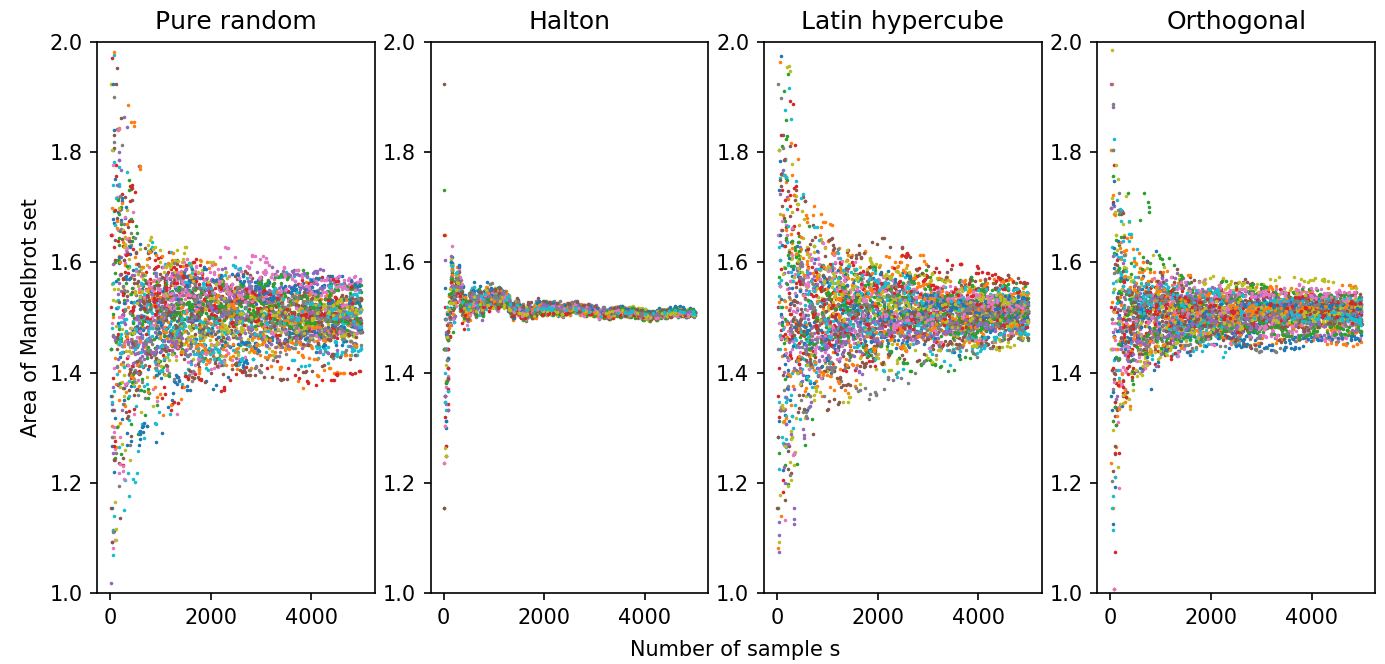
\includegraphics[width=\linewidth]{pictures/appendix/area_spread.png}
        \caption{Distribution of Area Results Based on Method}
        \label{fig:area_spread}
    \end{figure}

    \clearpage

    \section{Convergence of complex numbers in Mandelbrot set}
    \label{appendix:convergence_c}

    \begin{figure}[h]
        \centering
        \begin{subfigure}[t]{.47\linewidth}
            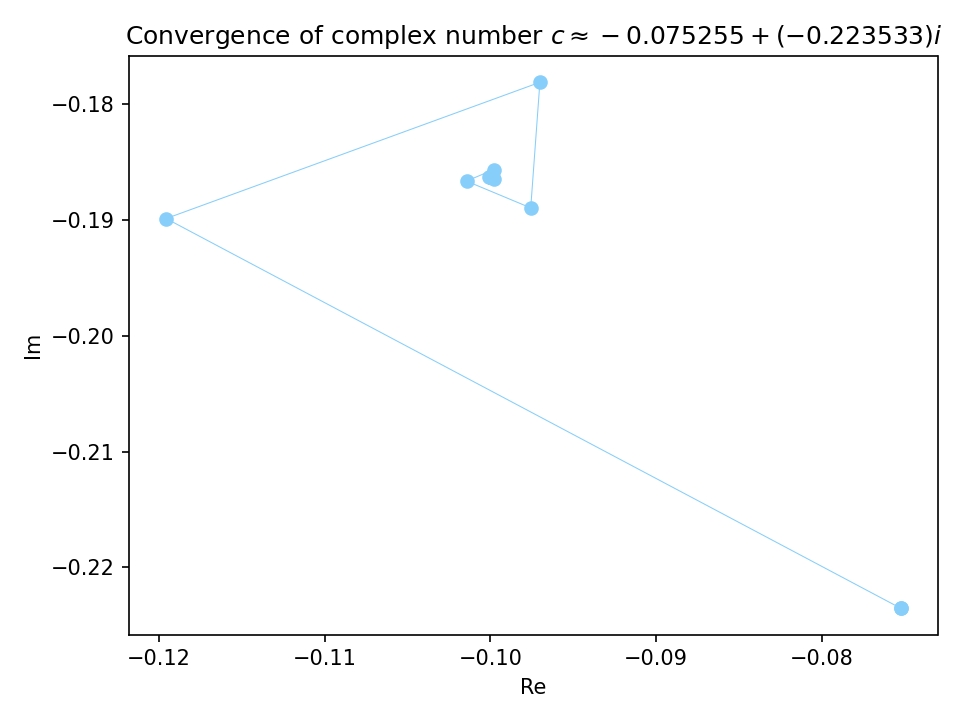
\includegraphics[width=\textwidth]{pictures/appendix/fast_convergence_2_c.png}
            \caption{Points far away from the boundaries of Mandelbrot set tends to converge fast. This point is located in the Main Cardioid.}
            \label{fig:complex_points_convergence_fast}
        \end{subfigure}
        \begin{subfigure}[t]{.47\linewidth}
            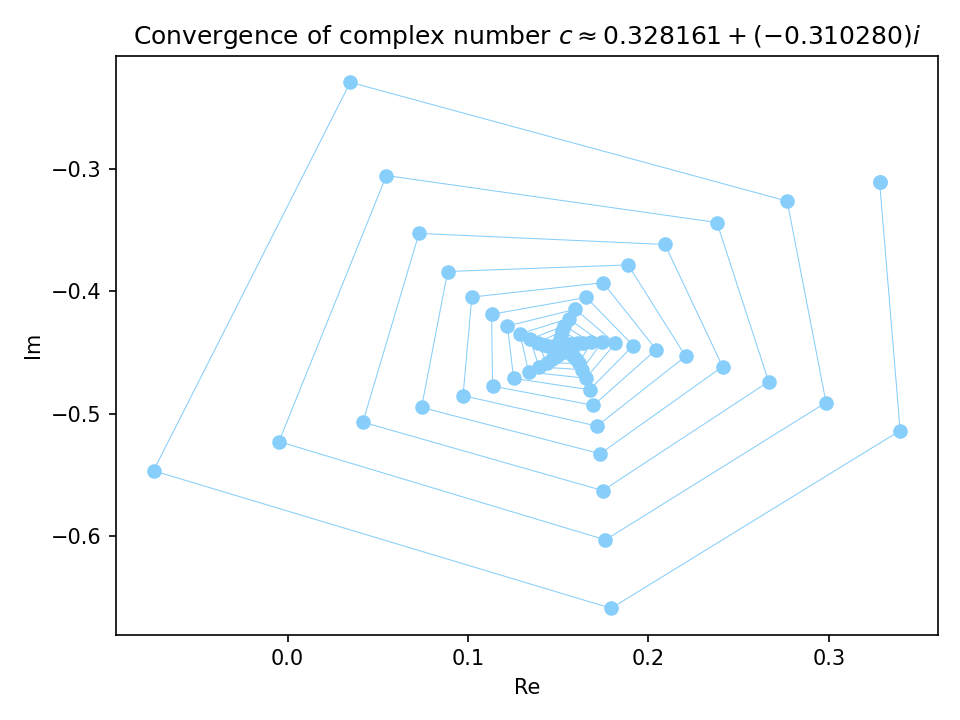
\includegraphics[width=\textwidth]{pictures/appendix/slow_convergence_c.png}
            \caption{Points closer to the boundaries of Mandelbrot set tends to converge slowly. This point is located near a boundary of the Main Cardioid.}
            \label{fig:complex_points_convergence_slow}
        \end{subfigure}

        \begin{subfigure}[t]{.47\linewidth}
            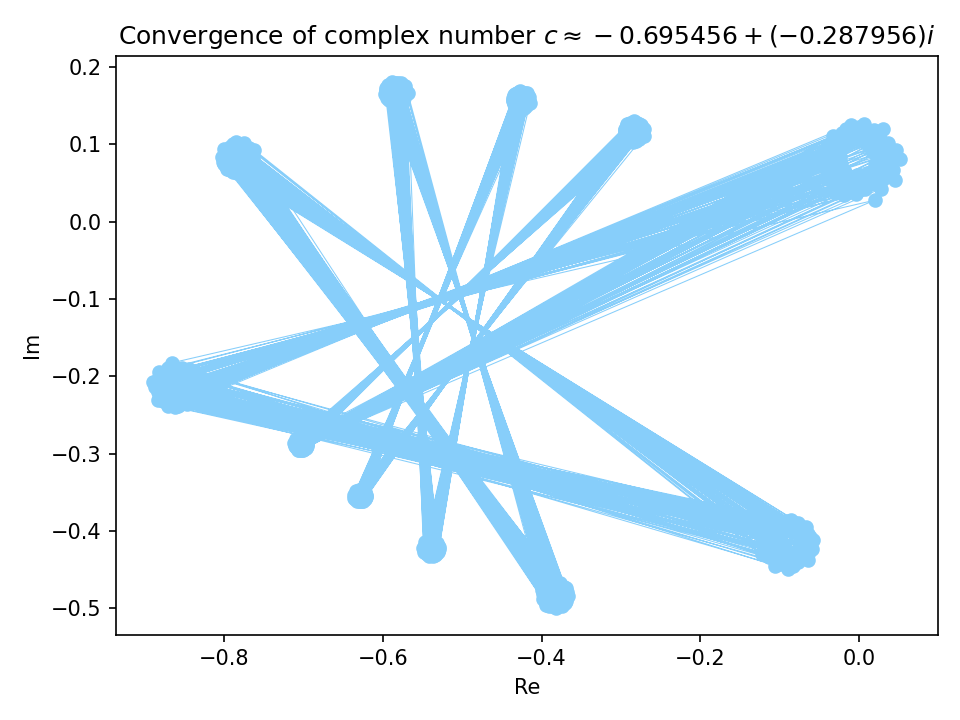
\includegraphics[width=\textwidth]{pictures/appendix/multiple_fixed_points_c.png}
            \caption{Complex numbers do not necessarily converge to a unique attractive fixed points. This point is located on the extreme border of the Main Cardioid, in the valley between the Main Cardioid and the First Bulb from the Mandelbrot set.}
            \label{fig:complex_points_convergence_multiple}
        \end{subfigure}
    \end{figure}

\end{document}